\documentclass[]{article}
\usepackage{lmodern}
\usepackage{amssymb,amsmath}
\usepackage{ifxetex,ifluatex}
\usepackage{fixltx2e} % provides \textsubscript
\ifnum 0\ifxetex 1\fi\ifluatex 1\fi=0 % if pdftex
  \usepackage[T1]{fontenc}
  \usepackage[utf8]{inputenc}
\else % if luatex or xelatex
  \ifxetex
    \usepackage{mathspec}
  \else
    \usepackage{fontspec}
  \fi
  \defaultfontfeatures{Ligatures=TeX,Scale=MatchLowercase}
\fi
% use upquote if available, for straight quotes in verbatim environments
\IfFileExists{upquote.sty}{\usepackage{upquote}}{}
% use microtype if available
\IfFileExists{microtype.sty}{%
\usepackage{microtype}
\UseMicrotypeSet[protrusion]{basicmath} % disable protrusion for tt fonts
}{}
\usepackage[margin=1in]{geometry}
\usepackage{hyperref}
\hypersetup{unicode=true,
            pdftitle={Processing, cleaning and saving NZ GREEN Grid project 1 minute electricity power data},
            pdfauthor={Ben Anderson (b.anderson@soton.ac.uk, @dataknut)},
            pdfborder={0 0 0},
            breaklinks=true}
\urlstyle{same}  % don't use monospace font for urls
\usepackage{color}
\usepackage{fancyvrb}
\newcommand{\VerbBar}{|}
\newcommand{\VERB}{\Verb[commandchars=\\\{\}]}
\DefineVerbatimEnvironment{Highlighting}{Verbatim}{commandchars=\\\{\}}
% Add ',fontsize=\small' for more characters per line
\usepackage{framed}
\definecolor{shadecolor}{RGB}{248,248,248}
\newenvironment{Shaded}{\begin{snugshade}}{\end{snugshade}}
\newcommand{\KeywordTok}[1]{\textcolor[rgb]{0.13,0.29,0.53}{\textbf{#1}}}
\newcommand{\DataTypeTok}[1]{\textcolor[rgb]{0.13,0.29,0.53}{#1}}
\newcommand{\DecValTok}[1]{\textcolor[rgb]{0.00,0.00,0.81}{#1}}
\newcommand{\BaseNTok}[1]{\textcolor[rgb]{0.00,0.00,0.81}{#1}}
\newcommand{\FloatTok}[1]{\textcolor[rgb]{0.00,0.00,0.81}{#1}}
\newcommand{\ConstantTok}[1]{\textcolor[rgb]{0.00,0.00,0.00}{#1}}
\newcommand{\CharTok}[1]{\textcolor[rgb]{0.31,0.60,0.02}{#1}}
\newcommand{\SpecialCharTok}[1]{\textcolor[rgb]{0.00,0.00,0.00}{#1}}
\newcommand{\StringTok}[1]{\textcolor[rgb]{0.31,0.60,0.02}{#1}}
\newcommand{\VerbatimStringTok}[1]{\textcolor[rgb]{0.31,0.60,0.02}{#1}}
\newcommand{\SpecialStringTok}[1]{\textcolor[rgb]{0.31,0.60,0.02}{#1}}
\newcommand{\ImportTok}[1]{#1}
\newcommand{\CommentTok}[1]{\textcolor[rgb]{0.56,0.35,0.01}{\textit{#1}}}
\newcommand{\DocumentationTok}[1]{\textcolor[rgb]{0.56,0.35,0.01}{\textbf{\textit{#1}}}}
\newcommand{\AnnotationTok}[1]{\textcolor[rgb]{0.56,0.35,0.01}{\textbf{\textit{#1}}}}
\newcommand{\CommentVarTok}[1]{\textcolor[rgb]{0.56,0.35,0.01}{\textbf{\textit{#1}}}}
\newcommand{\OtherTok}[1]{\textcolor[rgb]{0.56,0.35,0.01}{#1}}
\newcommand{\FunctionTok}[1]{\textcolor[rgb]{0.00,0.00,0.00}{#1}}
\newcommand{\VariableTok}[1]{\textcolor[rgb]{0.00,0.00,0.00}{#1}}
\newcommand{\ControlFlowTok}[1]{\textcolor[rgb]{0.13,0.29,0.53}{\textbf{#1}}}
\newcommand{\OperatorTok}[1]{\textcolor[rgb]{0.81,0.36,0.00}{\textbf{#1}}}
\newcommand{\BuiltInTok}[1]{#1}
\newcommand{\ExtensionTok}[1]{#1}
\newcommand{\PreprocessorTok}[1]{\textcolor[rgb]{0.56,0.35,0.01}{\textit{#1}}}
\newcommand{\AttributeTok}[1]{\textcolor[rgb]{0.77,0.63,0.00}{#1}}
\newcommand{\RegionMarkerTok}[1]{#1}
\newcommand{\InformationTok}[1]{\textcolor[rgb]{0.56,0.35,0.01}{\textbf{\textit{#1}}}}
\newcommand{\WarningTok}[1]{\textcolor[rgb]{0.56,0.35,0.01}{\textbf{\textit{#1}}}}
\newcommand{\AlertTok}[1]{\textcolor[rgb]{0.94,0.16,0.16}{#1}}
\newcommand{\ErrorTok}[1]{\textcolor[rgb]{0.64,0.00,0.00}{\textbf{#1}}}
\newcommand{\NormalTok}[1]{#1}
\usepackage{longtable,booktabs}
\usepackage{graphicx,grffile}
\makeatletter
\def\maxwidth{\ifdim\Gin@nat@width>\linewidth\linewidth\else\Gin@nat@width\fi}
\def\maxheight{\ifdim\Gin@nat@height>\textheight\textheight\else\Gin@nat@height\fi}
\makeatother
% Scale images if necessary, so that they will not overflow the page
% margins by default, and it is still possible to overwrite the defaults
% using explicit options in \includegraphics[width, height, ...]{}
\setkeys{Gin}{width=\maxwidth,height=\maxheight,keepaspectratio}
\IfFileExists{parskip.sty}{%
\usepackage{parskip}
}{% else
\setlength{\parindent}{0pt}
\setlength{\parskip}{6pt plus 2pt minus 1pt}
}
\setlength{\emergencystretch}{3em}  % prevent overfull lines
\providecommand{\tightlist}{%
  \setlength{\itemsep}{0pt}\setlength{\parskip}{0pt}}
\setcounter{secnumdepth}{5}
% Redefines (sub)paragraphs to behave more like sections
\ifx\paragraph\undefined\else
\let\oldparagraph\paragraph
\renewcommand{\paragraph}[1]{\oldparagraph{#1}\mbox{}}
\fi
\ifx\subparagraph\undefined\else
\let\oldsubparagraph\subparagraph
\renewcommand{\subparagraph}[1]{\oldsubparagraph{#1}\mbox{}}
\fi

%%% Use protect on footnotes to avoid problems with footnotes in titles
\let\rmarkdownfootnote\footnote%
\def\footnote{\protect\rmarkdownfootnote}

%%% Change title format to be more compact
\usepackage{titling}

% Create subtitle command for use in maketitle
\newcommand{\subtitle}[1]{
  \posttitle{
    \begin{center}\large#1\end{center}
    }
}

\setlength{\droptitle}{-2em}
  \title{Processing, cleaning and saving NZ GREEN Grid project 1 minute
electricity power data}
  \pretitle{\vspace{\droptitle}\centering\huge}
  \posttitle{\par}
  \author{Ben Anderson
(\href{mailto:b.anderson@soton.ac.uk}{\nolinkurl{b.anderson@soton.ac.uk}},
\texttt{@dataknut})}
  \preauthor{\centering\large\emph}
  \postauthor{\par}
  \predate{\centering\large\emph}
  \postdate{\par}
  \date{Last run at: 2018-06-05 13:00:47}


\begin{document}
\maketitle

{
\setcounter{tocdepth}{2}
\tableofcontents
}
\newpage

\section{Status}\label{status}

Full run using all data from /Volumes/hum-csafe/Research Projects/GREEN
Grid/\_RAW DATA/GridSpyData/

refreshData = 0 so re-using previous output. Should be relatively quick.

\section{Citation}\label{citation}

If you wish to use any of the material from this report please cite as:

\begin{itemize}
\tightlist
\item
  Anderson, B. (2018) Processing, cleaning and saving NZ GREEN Grid
  project 1 minute electricity power data, University of Otago: Dunedin,
  NZ.
\end{itemize}

\newpage

\section{Introduction}\label{introduction}

Report circulation:

\begin{itemize}
\tightlist
\item
  Restricted to:
  \href{https://www.otago.ac.nz/centre-sustainability/research/energy/otago050285.html}{NZ
  GREEN Grid} project partners and contractors.
\end{itemize}

\subsection{Purpose}\label{purpose}

This report is intended to:

\begin{itemize}
\tightlist
\item
  load and clean the project electricity power data (Grid Spy)
\item
  save the cleaned data out as a single file per household
\item
  produce summary data quality statistics
\end{itemize}

The resulting cleaned data has \emph{no} identifying information such as
names, addresses, email addresses, telephone numbers and is therefore
safe to share across all partners.

The data contains a unique household id which can be used to link it to
the NZ GREEN Grid time use diaries and dwelling/appliance surveys. With
some additional non-disclosure checks it should also be safe to archive
all of these linkable datasets for re-use via the UK
\href{http://reshare.ukdataservice.ac.uk/}{reshare} service.

\subsection{Requirements:}\label{requirements}

\begin{itemize}
\tightlist
\item
  grid spy 1 minute data downloads
\end{itemize}

\subsection{History}\label{history}

Generally tracked via our git.soton
\href{https://git.soton.ac.uk/ba1e12/nzGREENGrid}{repo}:

\begin{itemize}
\tightlist
\item
  \href{https://git.soton.ac.uk/ba1e12/nzGREENGrid/commits/master}{history}
\item
  \href{https://git.soton.ac.uk/ba1e12/nzGREENGrid/issues}{issues}
\end{itemize}

\subsection{Support}\label{support}

This work was supported by:

\begin{itemize}
\tightlist
\item
  The \href{https://www.otago.ac.nz/}{University of Otago}
\item
  The New Zealand \href{http://www.mbie.govt.nz/}{Ministry of Business,
  Innovation and Employment (MBIE)}
\item
  \href{http://www.energy.soton.ac.uk/tag/spatialec/}{SPATIALEC} - a
  \href{http://ec.europa.eu/research/mariecurieactions/about-msca/actions/if/index_en.htm}{Marie
  Skłodowska-Curie Global Fellowship} based at the University of Otago's
  \href{http://www.otago.ac.nz/centre-sustainability/staff/otago673896.html}{Centre
  for Sustainability} (2017-2019) \& the University of Southampton's
  Sustainable Energy Research Group (2019-202).
\end{itemize}

This work is (c) 2018 the University of Southampton.

We do not `support' the code but if you have a problem check the
\href{https://git.soton.ac.uk/ba1e12/nzGREENGrid/issues}{issues} on our
\href{https://git.soton.ac.uk/ba1e12/nzGREENGrid}{repo} and if it
doesn't already exist, open one. We might be able to fix it :-)

\section{Obtain listing of files}\label{obtain-listing-of-files}

In this section we generate a listing of all 1 minute data files that we
have received. If we are running over the complete dataset then we will
be using data from:

\begin{itemize}
\tightlist
\item
  /hum-csafe/Research Projects/GREEN Grid/\_RAW DATA/GridSpyData/
\end{itemize}

In this run we are using data from:

\begin{itemize}
\tightlist
\item
  /Volumes/hum-csafe/Research Projects/GREEN Grid/\_RAW
  DATA/GridSpyData/
\end{itemize}

If these do not match then this may be a test run.

\begin{verbatim}
## [1] "Re-using filelist"
\end{verbatim}

\begin{verbatim}
## [1] "Overall we have 22376 files from 44 households."
\end{verbatim}

Overall we have 22,376 files from 44 households. Of the 22,376, 13,080
(58.46\%) were \emph{not} loaded/checked as their file sizes indicated
that they contained no data.

\subsection{Date format checks}\label{date-format-checks}

We now need to check how many of the loaded files have an ambiguous or
default date - these could introduce errors.

\begin{longtable}[]{@{}llrll@{}}
\caption{Number of files and min/max date (as char) with given date
column names by inferred date format}\tabularnewline
\toprule
dateColName & dateFormat & nFiles & minDate & maxDate\tabularnewline
\midrule
\endfirsthead
\toprule
dateColName & dateFormat & nFiles & minDate & maxDate\tabularnewline
\midrule
\endhead
date NZ & dmy - definite & 1 & 27/03/2015 & 27/03/2015\tabularnewline
date NZ & mdy - definite & 2 & 5/26/2016 & 5/26/2016\tabularnewline
date NZ & ymd - default (but day/month value \textless{}= 12) & 12 &
2014-01-06 & 2016-06-07\tabularnewline
date NZ & ymd - definite & 67 & 2014-05-24 & 2016-07-13\tabularnewline
date UTC & ambiguous & 28 & 11-10-16 & 27/07/14\tabularnewline
date UTC & ymd - default (but day/month value \textless{}= 12) & 3607 &
2014-11-03 & 2018-05-12\tabularnewline
date UTC & ymd - definite & 5579 & 2015-03-26 &
2018-05-28\tabularnewline
unknown - do not load (fsize = 2751) & NA & 1812 & NA &
NA\tabularnewline
unknown - do not load (fsize = 43) & NA & 11268 & NA & NA\tabularnewline
\bottomrule
\end{longtable}

Results to note:

\begin{itemize}
\tightlist
\item
  There are 28 ambiguous files
\item
  The non-loaded files only have 2 distinct file sizes, confirming that
  they are unlikely to contain useful data.
\end{itemize}

We now inspect the ambiguous and (some of) the default files.

To help with data cleaning the following table lists files that have
ambiguous dates.

\begin{Shaded}
\begin{Highlighting}[]
\CommentTok{# list ambigious files}
\NormalTok{aList <-}\StringTok{ }\NormalTok{fListCompleteDT[dateFormat }\OperatorTok{==}\StringTok{ "ambiguous"}\NormalTok{, }
\NormalTok{                         .(file, dateColName, dateExample, dateFormat)]}

\NormalTok{cap <-}\StringTok{ }\KeywordTok{paste0}\NormalTok{(}\StringTok{"All "}\NormalTok{, }\KeywordTok{nrow}\NormalTok{(aList), }
              \StringTok{" files with an ambiguous dateFormat"}\NormalTok{)}

\NormalTok{knitr}\OperatorTok{::}\KeywordTok{kable}\NormalTok{(}\DataTypeTok{caption =}\NormalTok{ cap, aList)}
\end{Highlighting}
\end{Shaded}

\begin{longtable}[]{@{}llll@{}}
\caption{All 28 files with an ambiguous dateFormat}\tabularnewline
\toprule
file & dateColName & dateExample & dateFormat\tabularnewline
\midrule
\endfirsthead
\toprule
file & dateColName & dateExample & dateFormat\tabularnewline
\midrule
\endhead
rf\_06/15Jul2014-25May2016at1.csv & date UTC & 14/07/14 &
ambiguous\tabularnewline
rf\_07/15Jul2014-25May2016at1.csv & date UTC & 14/07/14 &
ambiguous\tabularnewline
rf\_08/15Jul2014-25May2016at1.csv & date UTC & 14/07/14 &
ambiguous\tabularnewline
rf\_10/15Jul2014-25May2016at1.csv & date UTC & 14/07/14 &
ambiguous\tabularnewline
rf\_11/15Jul2014-25May2016at1.csv & date UTC & 14/07/14 &
ambiguous\tabularnewline
rf\_13/15Jul2014-25May2016at1.csv & date UTC & 14/07/14 &
ambiguous\tabularnewline
rf\_19/15Jul2014-25May2016at1.csv & date UTC & 14/07/14 &
ambiguous\tabularnewline
rf\_21/15Jul2014-25May2016at1.csv & date UTC & 14/07/14 &
ambiguous\tabularnewline
rf\_22/15Jul2014-25May2016at1.csv & date UTC & 14/07/14 &
ambiguous\tabularnewline
rf\_23/15Jul2014-25May2016at1.csv & date UTC & 14/07/14 &
ambiguous\tabularnewline
rf\_24/15Jul2014-25May2016at1.csv & date UTC & 27/07/14 &
ambiguous\tabularnewline
rf\_25/12Oct2016-20Nov2017at1.csv & date UTC & 11-10-16 &
ambiguous\tabularnewline
rf\_26/15Jul2014-25May2016at1.csv & date UTC & 14/07/14 &
ambiguous\tabularnewline
rf\_27/15Jul2014-25May2016at1.csv & date UTC & 27/07/14 &
ambiguous\tabularnewline
rf\_29/24Mar2015-25May2016at1.csv & date UTC & 25/03/15 &
ambiguous\tabularnewline
rf\_30/15Feb2016-25May2016at1.csv & date UTC & 14/02/16 &
ambiguous\tabularnewline
rf\_30/24Mar2015-25May2016at1.csv & date UTC & 27/03/15 &
ambiguous\tabularnewline
rf\_31/24Mar2015-25May2016at1.csv & date UTC & 25/03/15 &
ambiguous\tabularnewline
rf\_34/18Jan2016-25May2016at1.csv & date UTC & 17/01/16 &
ambiguous\tabularnewline
rf\_34/20Jul2015-25May2016at1.csv & date UTC & 19/07/15 &
ambiguous\tabularnewline
rf\_34/24Mar2015-25May2016at1.csv & date UTC & 26/03/15 &
ambiguous\tabularnewline
rf\_35/24Mar2015-25May2016at1.csv & date UTC & 23/03/15 &
ambiguous\tabularnewline
rf\_39/24Mar2015-25May2016at1.csv & date UTC & 27/03/15 &
ambiguous\tabularnewline
rf\_43/24Mar2015-25May2016at1.csv & date UTC & 26/03/15 &
ambiguous\tabularnewline
rf\_43/27Mar2015-18Oct2015at1.csv & date UTC & 26/03/15 &
ambiguous\tabularnewline
rf\_44/24Mar2015-25May2016at1.csv & date UTC & 24/03/15 &
ambiguous\tabularnewline
rf\_46/12Oct2016-20Nov2017at1.csv & date UTC & 11-10-16 &
ambiguous\tabularnewline
rf\_47/24Mar2015-25May2016at1.csv & date UTC & 24/03/15 &
ambiguous\tabularnewline
\bottomrule
\end{longtable}

Check against file names to see what is reasonable and then fix them.

\begin{Shaded}
\begin{Highlighting}[]
\NormalTok{fListCompleteDT <-}\StringTok{ }\NormalTok{nzGREENGrid}\OperatorTok{::}\KeywordTok{fixAmbiguousDates}\NormalTok{(fListCompleteDT)}
\end{Highlighting}
\end{Shaded}

\begin{verbatim}
## [1] "Fixed 28 files with an ambiguous dateFormat"
\end{verbatim}

The following table lists up to 10 of the `date NZ' files which are set
by default - do they look OK to assume the default dateFormat? Compare
the file names with the dateExample\ldots{}

\begin{Shaded}
\begin{Highlighting}[]
\CommentTok{# list default files with NZ time}
\NormalTok{aList <-}\StringTok{ }\NormalTok{fListCompleteDT[dateColName }\OperatorTok{==}\StringTok{ "date NZ"} \OperatorTok{&}\StringTok{ }\NormalTok{dateFormat }\OperatorTok\StringTok{ "default"}\NormalTok{, }
\NormalTok{                         .(file, fSize, dateColName, dateExample, dateFormat)]}

\NormalTok{cap <-}\StringTok{ }\KeywordTok{paste0}\NormalTok{(}\StringTok{"First 10 (max) of "}\NormalTok{, }\KeywordTok{nrow}\NormalTok{(aList), }
              \StringTok{" files with dateColName = 'date NZ' and default dateFormat"}\NormalTok{)}

\NormalTok{knitr}\OperatorTok{::}\KeywordTok{kable}\NormalTok{(}\DataTypeTok{caption =}\NormalTok{ cap, }\KeywordTok{head}\NormalTok{(aList))}
\end{Highlighting}
\end{Shaded}

\begin{longtable}[]{@{}lrlll@{}}
\caption{First 10 (max) of 12 files with dateColName = `date NZ' and
default dateFormat}\tabularnewline
\toprule
file & fSize & dateColName & dateExample & dateFormat\tabularnewline
\midrule
\endfirsthead
\toprule
file & fSize & dateColName & dateExample & dateFormat\tabularnewline
\midrule
\endhead
rf\_01/1Jan2014-24May2014at1.csv & 6255737 & date NZ & 2014-01-06 & ymd
- default (but day/month value \textless{}= 12)\tabularnewline
rf\_02/1Jan2014-24May2014at1.csv & 6131625 & date NZ & 2014-03-03 & ymd
- default (but day/month value \textless{}= 12)\tabularnewline
rf\_06/24May2014-24May2015at1.csv & 19398444 & date NZ & 2014-06-09 &
ymd - default (but day/month value \textless{}= 12)\tabularnewline
rf\_10/24May2014-24May2015at1.csv & 24386048 & date NZ & 2014-07-09 &
ymd - default (but day/month value \textless{}= 12)\tabularnewline
rf\_11/24May2014-24May2015at1.csv & 23693893 & date NZ & 2014-07-08 &
ymd - default (but day/month value \textless{}= 12)\tabularnewline
rf\_12/24May2014-24May2015at1.csv & 21191785 & date NZ & 2014-07-09 &
ymd - default (but day/month value \textless{}= 12)\tabularnewline
\bottomrule
\end{longtable}

The following table lists up to 10 of the `date UTC' files which are set
by default - do they look OK to assume the default dateFormat? Compare
the file names with the dateExample\ldots{}

\begin{Shaded}
\begin{Highlighting}[]
\CommentTok{# list default files with UTC time}
\NormalTok{aList <-}\StringTok{ }\NormalTok{fListCompleteDT[dateColName }\OperatorTok{==}\StringTok{ "date UTC"} \OperatorTok{&}\StringTok{ }\NormalTok{dateFormat }\OperatorTok\StringTok{ "default"}\NormalTok{, }
\NormalTok{                         .(file, fSize, dateColName, dateExample, dateFormat)]}

\NormalTok{cap <-}\StringTok{ }\KeywordTok{paste0}\NormalTok{(}\StringTok{"First 10 (max) of "}\NormalTok{, }\KeywordTok{nrow}\NormalTok{(aList), }
              \StringTok{" files with dateColName = 'date UTC' and default dateFormat"}\NormalTok{)}

\NormalTok{knitr}\OperatorTok{::}\KeywordTok{kable}\NormalTok{(}\DataTypeTok{caption =}\NormalTok{ cap, }\KeywordTok{head}\NormalTok{(aList, }\DecValTok{10}\NormalTok{))}
\end{Highlighting}
\end{Shaded}

\begin{longtable}[]{@{}lrlll@{}}
\caption{First 10 (max) of 3607 files with dateColName = `date UTC' and
default dateFormat}\tabularnewline
\toprule
file & fSize & dateColName & dateExample & dateFormat\tabularnewline
\midrule
\endfirsthead
\toprule
file & fSize & dateColName & dateExample & dateFormat\tabularnewline
\midrule
\endhead
rf\_06/10Apr2018-11Apr2018at1.csv & 156944 & date UTC & 2018-04-09 & ymd
- default (but day/month value \textless{}= 12)\tabularnewline
rf\_06/10Dec2017-11Dec2017at1.csv & 156601 & date UTC & 2017-12-09 & ymd
- default (but day/month value \textless{}= 12)\tabularnewline
rf\_06/10Feb2018-11Feb2018at1.csv & 153353 & date UTC & 2018-02-09 & ymd
- default (but day/month value \textless{}= 12)\tabularnewline
rf\_06/10Jan2018-11Jan2018at1.csv & 153982 & date UTC & 2018-01-09 & ymd
- default (but day/month value \textless{}= 12)\tabularnewline
rf\_06/10Mar2018-11Mar2018at1.csv & 156471 & date UTC & 2018-03-09 & ymd
- default (but day/month value \textless{}= 12)\tabularnewline
rf\_06/10May2018-11May2018at1.csv & 156683 & date UTC & 2018-05-09 & ymd
- default (but day/month value \textless{}= 12)\tabularnewline
rf\_06/10Nov2017-11Nov2017at1.csv & 155639 & date UTC & 2017-11-09 & ymd
- default (but day/month value \textless{}= 12)\tabularnewline
rf\_06/11Apr2018-12Apr2018at1.csv & 157181 & date UTC & 2018-04-10 & ymd
- default (but day/month value \textless{}= 12)\tabularnewline
rf\_06/11Dec2017-12Dec2017at1.csv & 157814 & date UTC & 2017-12-10 & ymd
- default (but day/month value \textless{}= 12)\tabularnewline
rf\_06/11Feb2018-12Feb2018at1.csv & 153859 & date UTC & 2018-02-10 & ymd
- default (but day/month value \textless{}= 12)\tabularnewline
\bottomrule
\end{longtable}

Check final date formats:

\begin{longtable}[]{@{}llrll@{}}
\caption{Number of files \& min/max dates (as char) with given date
column names by final imputed date format}\tabularnewline
\toprule
dateColName & dateFormat & nFiles & minDate & maxDate\tabularnewline
\midrule
\endfirsthead
\toprule
dateColName & dateFormat & nFiles & minDate & maxDate\tabularnewline
\midrule
\endhead
date NZ & dmy - definite & 1 & 27/03/2015 & 27/03/2015\tabularnewline
date NZ & mdy - definite & 2 & 5/26/2016 & 5/26/2016\tabularnewline
date NZ & ymd - default (but day/month value \textless{}= 12) & 12 &
2014-01-06 & 2016-06-07\tabularnewline
date NZ & ymd - definite & 67 & 2014-05-24 & 2016-07-13\tabularnewline
date UTC & dmy - inferred & 28 & 11-10-16 & 27/07/14\tabularnewline
date UTC & ymd - default (but day/month value \textless{}= 12) & 3607 &
2014-11-03 & 2018-05-12\tabularnewline
date UTC & ymd - definite & 5579 & 2015-03-26 &
2018-05-28\tabularnewline
unknown - do not load (fsize = 2751) & NA & 1812 & NA &
NA\tabularnewline
unknown - do not load (fsize = 43) & NA & 11268 & NA & NA\tabularnewline
\bottomrule
\end{longtable}

\subsection{Data file quality checks}\label{data-file-quality-checks}

The following chart shows the distribution of these files over time
using their sizes. Note that white indicates the presence of small files
which may not contain observations.

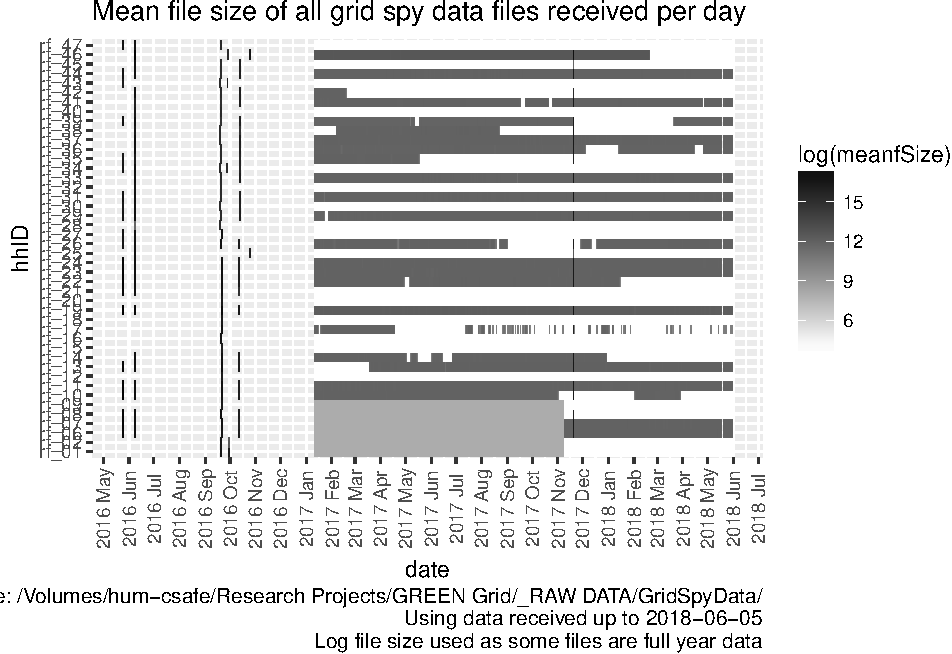
\includegraphics{processGridSpy1minData_files/figure-latex/allFileSizesPlot-1.pdf}

\begin{verbatim}
## Saving 6.5 x 4.5 in image
\end{verbatim}

The following chart shows the same chart but only for files which we
think contain data.

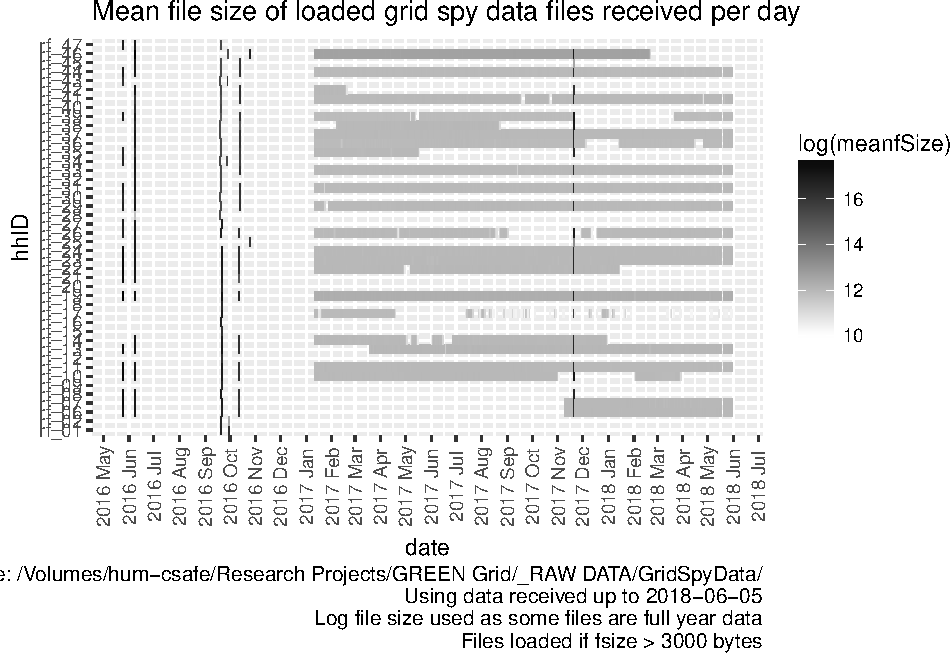
\includegraphics{processGridSpy1minData_files/figure-latex/loadedFileSizesPlot-1.pdf}

\begin{verbatim}
## Saving 6.5 x 4.5 in image
\end{verbatim}

\section{Load data files}\label{load-data-files}

\subsection{Grid Spy metadata}\label{grid-spy-metadata}

In this section we load metadata from /Users/ben/Syncplicity
Folders/Green Grid Project Management Folder/Gridspy/Master list of
Gridspy units.xlsx to link to the power data.

\begin{longtable}[]{@{}llllll@{}}
\caption{Meta data for sample}\tabularnewline
\toprule
sample & hhID & Adults & Teenagers & Children & removed\tabularnewline
\midrule
\endfirsthead
\toprule
sample & hhID & Adults & Teenagers & Children & removed\tabularnewline
\midrule
\endhead
Unison & rf\_28 & 2 & NA & 3(12,8,4) & NA\tabularnewline
Unison & rf\_29 & 2 & NA & 1 (7 months old) & live\tabularnewline
Unison & rf\_30 & 2 & 0 & 0 & NA\tabularnewline
Unison & rf\_31 & 2 (Plus cousin) & NA & NA & live\tabularnewline
Unison & rf\_32 & 2 & NA & 2 (7 and 4years old) & NA\tabularnewline
Unison & rf\_33 & 2 & 1(14yold) & 1 (6yold) & live\tabularnewline
Unison & rf\_34 & 3 & NA & NA & NA\tabularnewline
Unison & rf\_35 & 2 & NA & NA & 42322\tabularnewline
Unison & rf\_36 & 1 & 2 (14 and 12) & NA & live\tabularnewline
Unison & rf\_37 & 2 & NA & NA & live\tabularnewline
Unison & rf\_38 & NA & NA & NA & NA\tabularnewline
Unison & rf\_38 & 2 & NA & 2 (\textless{}12) & NA\tabularnewline
Unison & rf\_39 & 2 & 1 (16 YO) & NA & live\tabularnewline
Unison & rf\_40 & 2 & NA & NA & 42330\tabularnewline
Unison & rf\_41 & 2 & NA & 2 (11 and 8) & live\tabularnewline
Unison & rf\_42 & 2 & NA & 3 (\textless{}12 yold, 1 10 YO) &
NA\tabularnewline
Unison & rf\_43 & 2 & NA & NA & 42296\tabularnewline
Unison & rf\_44 & 2 & NA & 2 (10 and 7) & NA\tabularnewline
Unison & rf\_45 & 2 & NA & 3 (\textless{}12 years old) &
NA\tabularnewline
Unison & rf\_46 & 2 & NA & 1 (4yold-50\%) & live\tabularnewline
Unison & rf\_47 & 3 & 2 & NA & NA\tabularnewline
Powerco & rf\_12 & 1 & NA & NA & 3/6/1015\tabularnewline
Powerco & rf\_25 & 1 & NA & NA & NA\tabularnewline
Powerco & rf\_23 & 1 & NA & NA & NA\tabularnewline
Powerco & rf\_26 & 2 & NA & NA & NA\tabularnewline
Powerco & rf\_06 & 2 & NA & NA & NA\tabularnewline
Powerco & rf\_19 & 1 & NA & NA & NA\tabularnewline
Powerco & rf\_10 & 2 & NA & 1(3yo) & NA\tabularnewline
Powerco & rf\_11 & NA & NA & NA & NA\tabularnewline
Powerco & rf\_13 & 2 & 1(16yo) & 1(11) & NA\tabularnewline
Powerco & rf\_09 & 2 & NA & 1 & 42171\tabularnewline
Powerco & rf\_07 & 2 & NA & 2 & NA\tabularnewline
Powerco & rf\_22 & 2 & NA & NA & NA\tabularnewline
Powerco & rf\_08 & 2 & NA & NA & NA\tabularnewline
Powerco & rf\_18 & 2 & NA & 1(1yo) & 42532\tabularnewline
Powerco & rf\_17\_oldNo reused & 2 & 1(13yo) & 1(11yo) &
42457\tabularnewline
Powerco & rf\_14 & 1 & NA & 1 (11 yo) & NA\tabularnewline
Powerco & rf\_16 & 2 & NA & NA & 42089\tabularnewline
Powerco & rf\_21 & 2 & NA & NA & 42821\tabularnewline
Powerco & rf\_20 & 2 & NA & 2 & 42166\tabularnewline
Powerco & rf\_27 & 2 & 1 & 1 & NA\tabularnewline
Powerco & rf\_15\_old & 1 & NA & NA & 42019\tabularnewline
Powerco & rf\_24 & 2 & NA & 2 & NA\tabularnewline
Powerco & rf\_15 & NA & NA & NA & 42462\tabularnewline
Powerco & rf\_17 sn\_662 & NA & NA & NA & NA\tabularnewline
\bottomrule
\end{longtable}

\subsection{Grid Spy data}\label{grid-spy-data}

In this section we load the data files that have a file size
\textgreater{} 3000 bytes. Things to note:

\begin{itemize}
\tightlist
\item
  We assume that any files smaller than this value have no observations.
  This is based on:

  \begin{itemize}
  \tightlist
  \item
    Manual inspection of several small files
  \item
    The identical (small) file sizes involved
  \item
    \emph{But} we should probably test the first few lines to double
    check\ldots{}
  \end{itemize}
\item
  We have to deal with quite a lot of duplication some of which has
  caused the different date formats. See our
  \href{https://git.soton.ac.uk/ba1e12/nzGREENGrid/issues?scope=all\&utf8=\%E2\%9C\%93\&state=all}{repo
  issues list}.
\end{itemize}

The following table shows the number of files per household that we will
load.

\begin{Shaded}
\begin{Highlighting}[]
\CommentTok{# check files to load}
\NormalTok{t <-}\StringTok{ }\NormalTok{fListCompleteDT[dateColName }\OperatorTok\StringTok{ "do not load"}\NormalTok{, .(}\DataTypeTok{nFiles =}\NormalTok{ .N,}
                       \DataTypeTok{meanSize =} \KeywordTok{mean}\NormalTok{(fSize),}
                       \DataTypeTok{minFileDate =} \KeywordTok{min}\NormalTok{(fMDate),}
                       \DataTypeTok{maxFileDate =} \KeywordTok{max}\NormalTok{(fMDate)), keyby =}\StringTok{ }\NormalTok{.(hhID)]}

\NormalTok{knitr}\OperatorTok{::}\KeywordTok{kable}\NormalTok{(}\DataTypeTok{caption =} \StringTok{"Summary of household files to load"}\NormalTok{, t)}
\end{Highlighting}
\end{Shaded}

\begin{longtable}[]{@{}lrrll@{}}
\caption{Summary of household files to load}\tabularnewline
\toprule
hhID & nFiles & meanSize & minFileDate & maxFileDate\tabularnewline
\midrule
\endfirsthead
\toprule
hhID & nFiles & meanSize & minFileDate & maxFileDate\tabularnewline
\midrule
\endhead
rf\_01 & 506 & 1659.237 & 2017-01-11 & 2018-05-30\tabularnewline
rf\_02 & 506 & 1659.237 & 2017-01-11 & 2018-05-30\tabularnewline
rf\_06 & 302 & 2751.000 & 2017-01-11 & 2017-11-08\tabularnewline
rf\_07 & 302 & 2751.000 & 2017-01-11 & 2017-11-08\tabularnewline
rf\_08 & 505 & 1662.438 & 2017-01-11 & 2018-05-30\tabularnewline
rf\_09 & 506 & 1659.237 & 2017-01-11 & 2018-05-30\tabularnewline
rf\_10 & 152 & 43.000 & 2017-11-03 & 2018-05-30\tabularnewline
rf\_12 & 506 & 43.000 & 2017-01-11 & 2018-05-30\tabularnewline
rf\_13 & 68 & 43.000 & 2017-01-11 & 2017-03-18\tabularnewline
rf\_14 & 180 & 43.000 & 2017-05-04 & 2018-05-30\tabularnewline
rf\_15 & 506 & 43.000 & 2017-01-11 & 2018-05-30\tabularnewline
rf\_16 & 506 & 43.000 & 2017-01-11 & 2018-05-30\tabularnewline
rf\_17 & 296 & 43.000 & 2017-01-18 & 2018-05-28\tabularnewline
rf\_18 & 506 & 43.000 & 2017-01-11 & 2018-05-30\tabularnewline
rf\_20 & 506 & 43.000 & 2017-01-11 & 2018-05-30\tabularnewline
rf\_21 & 506 & 43.000 & 2017-01-11 & 2018-05-30\tabularnewline
rf\_22 & 139 & 43.000 & 2017-05-01 & 2018-05-30\tabularnewline
rf\_25 & 505 & 43.000 & 2017-01-11 & 2018-05-30\tabularnewline
rf\_26 & 94 & 43.000 & 2017-08-21 & 2017-12-17\tabularnewline
rf\_27 & 506 & 43.000 & 2017-01-11 & 2018-05-30\tabularnewline
rf\_28 & 506 & 43.000 & 2017-01-11 & 2018-05-30\tabularnewline
rf\_29 & 3 & 43.000 & 2017-01-25 & 2017-01-27\tabularnewline
rf\_30 & 506 & 43.000 & 2017-01-11 & 2018-05-30\tabularnewline
rf\_32 & 506 & 43.000 & 2017-01-11 & 2018-05-30\tabularnewline
rf\_34 & 506 & 43.000 & 2017-01-11 & 2018-05-30\tabularnewline
rf\_35 & 376 & 43.000 & 2017-05-19 & 2018-05-30\tabularnewline
rf\_36 & 49 & 43.000 & 2017-12-06 & 2018-04-26\tabularnewline
rf\_38 & 308 & 43.000 & 2017-01-11 & 2018-05-30\tabularnewline
rf\_39 & 124 & 43.000 & 2017-05-14 & 2018-03-20\tabularnewline
rf\_40 & 506 & 43.000 & 2017-01-11 & 2018-05-30\tabularnewline
rf\_41 & 8 & 43.000 & 2017-09-19 & 2018-04-27\tabularnewline
rf\_42 & 464 & 43.000 & 2017-02-20 & 2018-05-30\tabularnewline
rf\_43 & 506 & 43.000 & 2017-01-11 & 2018-05-30\tabularnewline
rf\_45 & 505 & 43.000 & 2017-01-11 & 2018-05-30\tabularnewline
rf\_46 & 98 & 43.000 & 2018-02-22 & 2018-05-30\tabularnewline
rf\_47 & 506 & 43.000 & 2017-01-11 & 2018-05-30\tabularnewline
\bottomrule
\end{longtable}

Now load, clean and save the valid data giving feedback where
appropriate.

\begin{Shaded}
\begin{Highlighting}[]
\CommentTok{# process the data & update the fListCompleteDT}
\CommentTok{# get a few rows of data as an example}
\CommentTok{# refresh the data depending on refreshData (set in ./setup.R)}

\ControlFlowTok{if}\NormalTok{(refreshData)\{}
  \KeywordTok{print}\NormalTok{(}\KeywordTok{paste0}\NormalTok{(}\StringTok{"'refreshData' = "}\NormalTok{, refreshData, }\StringTok{" so re-building filelist"}\NormalTok{))}
  \CommentTok{# returns the updated file list into fListCompleteDT}
  \CommentTok{# creates hhStatDT (used below)}
  \CommentTok{# puts top 6 rows of last file into lastOfHeadDT}
\NormalTok{  fListCompleteDT <-}\StringTok{ }\NormalTok{nzGREENGrid}\OperatorTok{::}\KeywordTok{processGridSpyDataFiles}\NormalTok{(fListCompleteDT, fListFinal)}
\NormalTok{\} }\ControlFlowTok{else}\NormalTok{ \{}
  \KeywordTok{print}\NormalTok{(}\KeywordTok{paste0}\NormalTok{(}\StringTok{"'refreshData' = "}\NormalTok{, refreshData, }\StringTok{" so re-using filelist"}\NormalTok{))}
\NormalTok{  fListCompleteDT <-}\StringTok{ }\KeywordTok{fread}\NormalTok{(}\KeywordTok{paste0}\NormalTok{(outPath,fListFinal))}
  
  \CommentTok{# need to create hhStatDT}
\NormalTok{  ofile <-}\StringTok{ }\KeywordTok{paste0}\NormalTok{(outPath, }\StringTok{"hhDailyObservationsStats.csv"}\NormalTok{)}
\NormalTok{  hhStatDT <-}\StringTok{ }\KeywordTok{fread}\NormalTok{(ofile)}
  
  \CommentTok{# need to get lastOfHeadDT}
  \CommentTok{# do this by getting the first in the processed list}
\NormalTok{  dPath <-}\StringTok{ }\KeywordTok{paste0}\NormalTok{(outPath,}\StringTok{"data/"}\NormalTok{)}
\NormalTok{  fList <-}\StringTok{ }\KeywordTok{list.files}\NormalTok{(}\DataTypeTok{path =}\NormalTok{ dPath, }\DataTypeTok{pattern =} \StringTok{"csv.gz"}\NormalTok{)}
  \KeywordTok{print}\NormalTok{(}\KeywordTok{paste0}\NormalTok{(}\StringTok{"Re-using saved data file..."}\NormalTok{))}
\NormalTok{  lastOfHeadDT <-}\StringTok{ }\KeywordTok{head}\NormalTok{(}\KeywordTok{read_csv}\NormalTok{(}\KeywordTok{paste0}\NormalTok{(dPath, fList[}\DecValTok{1}\NormalTok{])))}
\NormalTok{\}}
\end{Highlighting}
\end{Shaded}

\begin{verbatim}
## [1] "'refreshData' = 0 so re-using filelist"
## [1] "Re-using saved data file..."
\end{verbatim}

\begin{verbatim}
## Parsed with column specification:
## cols(
##   hhID = col_character(),
##   r_dateTime = col_datetime(format = ""),
##   circuit = col_character(),
##   powerW = col_double()
## )
\end{verbatim}

\begin{Shaded}
\begin{Highlighting}[]
\CommentTok{# test}
\KeywordTok{kable}\NormalTok{(}\DataTypeTok{caption =} \StringTok{"Example data rows"}\NormalTok{, lastOfHeadDT)}
\end{Highlighting}
\end{Shaded}

\begin{longtable}[]{@{}lllr@{}}
\caption{Example data rows}\tabularnewline
\toprule
hhID & r\_dateTime & circuit & powerW\tabularnewline
\midrule
\endfirsthead
\toprule
hhID & r\_dateTime & circuit & powerW\tabularnewline
\midrule
\endhead
rf\_01 & 2014-01-06 03:03:00 & Kitchen power\$1632 &
45.58\tabularnewline
rf\_01 & 2014-01-06 03:04:00 & Kitchen power\$1632 &
45.58\tabularnewline
rf\_01 & 2014-03-07 02:56:00 & Kitchen power\$1632 &
45.58\tabularnewline
rf\_01 & 2014-03-07 02:57:00 & Kitchen power\$1632 &
54.13\tabularnewline
rf\_01 & 2014-03-07 02:58:00 & Kitchen power\$1632 &
136.26\tabularnewline
rf\_01 & 2014-03-07 02:59:00 & Kitchen power\$1632 &
141.96\tabularnewline
\bottomrule
\end{longtable}

\section{Data quality analysis}\label{data-quality-analysis}

Now produce some data quality plots \& tables.

\subsection{Circuit label checks}\label{circuit-label-checks}

The following table shows the number of data files with different
circuit labels by household. In theory there should only be one unique
list per household and it should be present in every data file. If this
is not the case then this implies that:

\begin{itemize}
\tightlist
\item
  some of the circuit labels for these households may have been changed
  during the data collection process;
\item
  some of the circuit labels may have character conversion errors which
  have changed the labels during the data collection process;
\item
  at least one file from one household has been saved to a folder
  containing data from a different household (unfortunately the raw data
  files do \emph{not} contain household IDs in the data or the file
  names which would enable checking/preventative filtering). This will
  be visible in the table if two households appear to share
  \emph{exactly} the same list of circuit labels.
\end{itemize}

Some or all of these may be true at any given time!

\begin{quote}
NB: This table is only legible in the html version of this report
because latex does a very bad job of wrapping table cell text. A version
is saved in /Volumes/hum-csafe/Research Projects/GREEN
Grid/Clean\_data/safe/gridSpy/1min/circuitLabelCheck.csv for viewing in
e.g.~xl.
\end{quote}

\begin{longtable}[]{@{}lrrrrrrrrrrrrrrrrrrrrrrrrrrrrrrrrrrrrrrrrrrrr@{}}
\caption{Circuit labels list by household}\tabularnewline
\toprule
& rf\_06 & rf\_07 & rf\_08 & rf\_09 & rf\_10 & rf\_11 & rf\_12 & rf\_13
& rf\_14 & rf\_15 & rf\_15\_old & rf\_16 & rf\_17 sn\_662 &
rf\_17\_oldNo reused & rf\_18 & rf\_19 & rf\_20 & rf\_21 & rf\_22 &
rf\_23 & rf\_24 & rf\_25 & rf\_26 & rf\_27 & rf\_28 & rf\_29 & rf\_30 &
rf\_31 & rf\_32 & rf\_33 & rf\_34 & rf\_35 & rf\_36 & rf\_37 & rf\_38 &
rf\_39 & rf\_40 & rf\_41 & rf\_42 & rf\_43 & rf\_44 & rf\_45 & rf\_46 &
rf\_47\tabularnewline
\midrule
\endfirsthead
\toprule
& rf\_06 & rf\_07 & rf\_08 & rf\_09 & rf\_10 & rf\_11 & rf\_12 & rf\_13
& rf\_14 & rf\_15 & rf\_15\_old & rf\_16 & rf\_17 sn\_662 &
rf\_17\_oldNo reused & rf\_18 & rf\_19 & rf\_20 & rf\_21 & rf\_22 &
rf\_23 & rf\_24 & rf\_25 & rf\_26 & rf\_27 & rf\_28 & rf\_29 & rf\_30 &
rf\_31 & rf\_32 & rf\_33 & rf\_34 & rf\_35 & rf\_36 & rf\_37 & rf\_38 &
rf\_39 & rf\_40 & rf\_41 & rf\_42 & rf\_43 & rf\_44 & rf\_45 & rf\_46 &
rf\_47\tabularnewline
\midrule
\endhead
Bed 2, 2nd Fridge\$2828, Heat Pump\$2826, Hot Water - Controlled\$2825,
Incomer - Uncontrolled\$2824, Kitchen, Laundry \& Beds 1\&3\$2829, Oven
\& Oven Wall Appliances\$2827 & 0 & 0 & 0 & 0 & 0 & 0 & 0 & 0 & 0 & 0 &
0 & 0 & 0 & 0 & 0 & 0 & 0 & 0 & 0 & 0 & 0 & 0 & 0 & 3 & 0 & 0 & 0 & 0 &
0 & 0 & 0 & 0 & 0 & 0 & 0 & 0 & 0 & 0 & 0 & 0 & 0 & 0 & 0 &
0\tabularnewline
Bedroom \& Lounge Heat Pumps\$2741, Incomer 1 - All\$2738, Incomer 2 -
All\$2737, Kitchen Appliances\$2735, Laundry\$2734, Oven\$2736, PV
1\$2739, PV 2\$2733, Theatre Heat Pump\$2740 & 0 & 0 & 0 & 0 & 0 & 0 & 0
& 0 & 0 & 0 & 0 & 0 & 0 & 0 & 0 & 508 & 0 & 0 & 0 & 0 & 0 & 0 & 0 & 0 &
0 & 0 & 0 & 0 & 0 & 0 & 0 & 0 & 0 & 0 & 0 & 0 & 0 & 0 & 0 & 0 & 0 & 0 &
0 & 0\tabularnewline
Bedrooms \& Lounge\$2602, Heat Pump\$2598, Incomer - All\$2599, Kitchen
Appliances\$2601, Laundry \& Garage\$2597, Oven\$2600 & 0 & 0 & 0 & 0 &
358 & 0 & 0 & 0 & 0 & 0 & 0 & 0 & 0 & 0 & 0 & 0 & 0 & 0 & 0 & 0 & 0 & 0
& 0 & 0 & 0 & 0 & 0 & 0 & 0 & 0 & 0 & 0 & 0 & 0 & 0 & 0 & 0 & 0 & 0 & 0
& 0 & 0 & 0 & 0\tabularnewline
Downstairs (inc 1 Heat Pump)\$2212, Hot Water - Controlled\$2208,
Incomer - Uncontrolled\$2209, Kitchen \& Laundry\$2213, Oven \&
Hob\$2210, Upstairs Heat Pumps\$2211 & 0 & 0 & 0 & 0 & 0 & 0 & 0 & 440 &
0 & 0 & 0 & 0 & 0 & 0 & 0 & 0 & 0 & 0 & 0 & 0 & 0 & 0 & 0 & 0 & 0 & 0 &
0 & 0 & 0 & 0 & 0 & 0 & 0 & 0 & 0 & 0 & 0 & 0 & 0 & 0 & 0 & 0 & 0 &
0\tabularnewline
Fridge\$2752, Heat Pump \& Washing Machine\$2750, Incomer - All\$2748,
Kitchen Appliances \& Garage\$2753, Lower Bedrooms \& Bathrooms\$2751,
Oven\$2749 & 0 & 0 & 0 & 0 & 0 & 0 & 0 & 0 & 0 & 0 & 0 & 0 & 0 & 0 & 0 &
0 & 0 & 4 & 0 & 0 & 0 & 0 & 0 & 0 & 0 & 0 & 0 & 0 & 0 & 0 & 0 & 0 & 0 &
0 & 0 & 0 & 0 & 0 & 0 & 0 & 0 & 0 & 0 & 0\tabularnewline
Hallway \& Washing Machine\$2683, Hot Water - Controlled\$2679, Incomer
1 - Uncont inc Oven\$2681, Incomer 2 - Uncont inc Stove\$2680, Kitchen
Appliances \& Bedrooms\$2684, Microwave \& Breadmaker\$2682 & 0 & 0 & 0
& 0 & 0 & 0 & 0 & 0 & 0 & 0 & 0 & 1 & 0 & 0 & 0 & 0 & 0 & 0 & 0 & 0 & 0
& 0 & 0 & 0 & 0 & 0 & 0 & 0 & 0 & 0 & 0 & 0 & 0 & 0 & 0 & 0 & 0 & 0 & 0
& 0 & 0 & 0 & 0 & 0\tabularnewline
Heat Pump (x2) \& Lounge Power\$4166, Hot Water - Controlled\$4167,
Incomer - Uncontrolled\$4168, Kitchen Appliances\$4163, Laundry\$4164,
Lighting\$4165 & 0 & 0 & 0 & 0 & 0 & 0 & 0 & 0 & 0 & 0 & 0 & 0 & 0 & 0 &
0 & 0 & 0 & 0 & 0 & 0 & 0 & 0 & 0 & 0 & 0 & 0 & 0 & 0 & 0 & 0 & 0 & 0 &
0 & 0 & 0 & 0 & 2 & 0 & 0 & 0 & 0 & 0 & 0 & 0\tabularnewline
Heat Pump \& 2 x Bathroom Heat\$4171, Incomer - All\$4170, Kitchen Power
\& Heat, Lounge\$4174, Laundry, Garage \& 2 Bedrooms\$4173,
Lighting\$4172, Wall Oven\$4169 & 0 & 0 & 0 & 0 & 0 & 0 & 0 & 0 & 0 & 0
& 0 & 0 & 0 & 0 & 0 & 0 & 0 & 0 & 0 & 0 & 0 & 0 & 0 & 0 & 0 & 0 & 0 & 0
& 0 & 0 & 0 & 0 & 0 & 0 & 0 & 0 & 0 & 0 & 0 & 0 & 0 & 0 & 0 &
3\tabularnewline
Heat Pump \& Bedroom 2\$2731, Incomer 1 - Uncont - Inc Hob\$2729,
Incomer 2 - Uncont - Inc Oven\$2730, Kitchen Appliances\$2727,
Laundry\$2732, Lounge, Dining \& Bedrooms\$2728 & 0 & 0 & 0 & 2 & 0 & 0
& 0 & 0 & 0 & 0 & 0 & 0 & 0 & 0 & 0 & 0 & 0 & 0 & 0 & 0 & 0 & 0 & 0 & 0
& 0 & 0 & 0 & 0 & 0 & 0 & 0 & 0 & 0 & 0 & 0 & 0 & 0 & 0 & 0 & 0 & 0 & 0
& 0 & 0\tabularnewline
Heat Pump \& Kitchen Appliances\$4186, Hot Water - Controlled\$4184,
Incomer - Uncontrolled\$4181, Laundry\$4185, Lighting\$4183, Oven\$4182
& 0 & 0 & 0 & 0 & 0 & 0 & 0 & 0 & 0 & 0 & 0 & 0 & 0 & 0 & 0 & 0 & 0 & 0
& 0 & 0 & 0 & 0 & 0 & 0 & 0 & 505 & 0 & 0 & 0 & 0 & 0 & 0 & 0 & 0 & 0 &
0 & 0 & 0 & 0 & 0 & 0 & 0 & 0 & 0\tabularnewline
Heat Pump \& Lounge\$2590, Hob\$2589, Hot Water Cpbd Heater- Cont\$2586,
Incomer - Uncontrolled\$2585, Kitchen Appliances \& Laundry\$2588, Spa -
Uncontrolled\$2587 & 0 & 0 & 0 & 0 & 0 & 508 & 0 & 0 & 0 & 0 & 0 & 0 & 0
& 0 & 0 & 0 & 0 & 0 & 0 & 0 & 0 & 0 & 0 & 0 & 0 & 0 & 0 & 0 & 0 & 0 & 0
& 0 & 0 & 0 & 0 & 0 & 0 & 0 & 0 & 0 & 0 & 0 & 0 & 0\tabularnewline
Heat Pump \& Misc\$2107, Hob\$2109, Hot Water - Controlled\$2110,
Incomer 1 - Uncontrolled\$2112, Incomer 2 - Uncontrolled\$2111, Oven \&
Kitchen Appliances\$2108 & 0 & 0 & 0 & 0 & 0 & 0 & 0 & 0 & 0 & 0 & 0 & 0
& 0 & 0 & 0 & 0 & 2 & 0 & 0 & 0 & 0 & 0 & 0 & 0 & 0 & 0 & 0 & 0 & 0 & 0
& 0 & 0 & 0 & 0 & 0 & 0 & 0 & 0 & 0 & 0 & 0 & 0 & 0 & 0\tabularnewline
Heat Pump\$2092, Hot Water - Controlled\$2094, Incomer -
Uncontrolled\$2093, Kitchen\$2089, Laundry \& 2nd Fridge Freezer\$2090,
Oven \& Hob\$2091 & 0 & 0 & 5 & 0 & 0 & 0 & 0 & 0 & 0 & 0 & 0 & 0 & 0 &
0 & 0 & 0 & 0 & 0 & 0 & 0 & 0 & 0 & 0 & 0 & 0 & 0 & 0 & 0 & 0 & 0 & 0 &
0 & 0 & 0 & 0 & 0 & 0 & 0 & 0 & 0 & 0 & 0 & 0 & 0\tabularnewline
Heat Pump\$2758, Hob \& Kitchen Appliances\$2759, Hot Water -
Controlled\$2761, Incomer 1 - Uncontrolled \$2763, Incomer 1 -
Uncontrolled\$2757, Incomer 2 - Uncontrolled \$2762, Oven\$2760 & 0 & 0
& 0 & 0 & 0 & 0 & 0 & 0 & 0 & 0 & 0 & 0 & 0 & 0 & 0 & 0 & 0 & 0 & 0 & 0
& 0 & 1 & 0 & 0 & 0 & 0 & 0 & 0 & 0 & 0 & 0 & 0 & 0 & 0 & 0 & 0 & 0 & 0
& 0 & 0 & 0 & 0 & 0 & 0\tabularnewline
Heat Pump\$2758, Hob \& Kitchen Appliances\$2759, Hot Water -
Controlled\$2761, Incomer 1 - Uncontrolled \$2763, Incomer 2 -
Uncontrolled \$2762, Oven\$2760 & 0 & 0 & 0 & 0 & 0 & 0 & 0 & 0 & 0 & 0
& 0 & 0 & 0 & 0 & 0 & 0 & 0 & 0 & 0 & 0 & 0 & 2 & 0 & 0 & 0 & 0 & 0 & 0
& 0 & 0 & 0 & 0 & 0 & 0 & 0 & 0 & 0 & 0 & 0 & 0 & 0 & 0 & 0 &
0\tabularnewline
Heat Pump\$4124, Hot Water - Uncontrolled\$4125, Incomer -
Uncontrolled\$4126, Kitchen Appliances\$4121, Laundry, Garage Fridge
Freezer\$4122, Lighting\$4123 & 0 & 0 & 0 & 0 & 0 & 0 & 0 & 0 & 0 & 0 &
0 & 0 & 0 & 0 & 0 & 0 & 0 & 0 & 0 & 0 & 0 & 0 & 0 & 0 & 0 & 0 & 0 & 0 &
0 & 0 & 0 & 134 & 0 & 0 & 0 & 0 & 0 & 0 & 0 & 0 & 0 & 0 & 0 &
0\tabularnewline
Heat Pump\$4130, Hot Water - Uncontrolled\$4131, Incomer - All\$4132,
Kitchen Appliances\$4127, Laundry \& Freezer\$4128, Lighting (inc heat
lamps)\$4129 & 0 & 0 & 0 & 0 & 0 & 0 & 0 & 0 & 0 & 0 & 0 & 0 & 0 & 0 & 0
& 0 & 0 & 0 & 0 & 0 & 0 & 0 & 0 & 0 & 0 & 0 & 0 & 0 & 0 & 0 & 0 & 0 & 0
& 0 & 0 & 0 & 0 & 0 & 45 & 0 & 0 & 0 & 0 & 0\tabularnewline
Heat Pump\$4134, Hot Water - Controlled\$4135, Incomer
-Uncontrolled\$4136, Kitchen Appliances\$4137, Laundry \& Fridge
Freezer\$4138, Lighting\$4133 & 0 & 0 & 0 & 0 & 0 & 0 & 0 & 0 & 0 & 0 &
0 & 0 & 0 & 0 & 0 & 0 & 0 & 0 & 0 & 0 & 0 & 0 & 0 & 0 & 0 & 0 & 0 & 0 &
0 & 0 & 0 & 0 & 0 & 507 & 0 & 0 & 0 & 0 & 0 & 0 & 0 & 0 & 0 &
0\tabularnewline
Heat Pump\$4150, Hot Water - Uncontrolled\$4147, Incomer - All\$4148,
Kitchen Appliances\$4145, Lighting\$4149, Washing Machine\$4146 & 0 & 0
& 0 & 0 & 0 & 0 & 0 & 0 & 0 & 0 & 0 & 0 & 0 & 0 & 0 & 0 & 0 & 0 & 0 & 0
& 0 & 0 & 0 & 0 & 0 & 0 & 0 & 0 & 0 & 0 & 0 & 0 & 458 & 0 & 0 & 0 & 0 &
0 & 0 & 0 & 0 & 0 & 0 & 0\tabularnewline
Heat Pump\$4154, Hot Water - Controlled\$4155, Incomer -
Uncontrolled\$4156, Kitchen Appliances\$4151, Laundry \$4152,
Lighting\$4153 & 0 & 0 & 0 & 0 & 0 & 0 & 0 & 0 & 0 & 0 & 0 & 0 & 0 & 0 &
0 & 0 & 0 & 0 & 0 & 0 & 0 & 0 & 0 & 0 & 0 & 0 & 0 & 0 & 0 & 0 & 0 & 0 &
0 & 0 & 0 & 0 & 0 & 0 & 0 & 0 & 508 & 0 & 0 & 0\tabularnewline
Heat Pump\$4160, Hot Water - Controlled\$4158, Incomer -
Uncontrolled\$4157, Kitchen Appliances\$4161, Laundry \& Garage
Fridge\$4162, Lighting\$4159 & 0 & 0 & 0 & 0 & 0 & 0 & 0 & 0 & 0 & 0 & 0
& 0 & 0 & 0 & 0 & 0 & 0 & 0 & 0 & 0 & 0 & 0 & 0 & 0 & 0 & 0 & 0 & 0 & 0
& 0 & 0 & 0 & 0 & 0 & 0 & 0 & 0 & 0 & 0 & 0 & 0 & 4 & 0 &
0\tabularnewline
Heat Pump\$4175, Hot Water - Controlled\$4178, Incomer -
Uncontrolled\$4177, Kitchen, Dining \& Office\$4179, Laundry, Lounge,
Garage, Bed\$4180, Lighting\$4176 & 0 & 0 & 0 & 0 & 0 & 0 & 0 & 0 & 0 &
0 & 0 & 0 & 0 & 0 & 0 & 0 & 0 & 0 & 0 & 0 & 0 & 0 & 0 & 0 & 0 & 0 & 0 &
0 & 0 & 0 & 0 & 0 & 0 & 0 & 402 & 0 & 0 & 0 & 0 & 0 & 0 & 0 & 0 &
0\tabularnewline
Heat Pump\$4190, Incomer - All\$4192, Kitchen Appliances\$4187,
Laundry\$4188, Lighting\$4189, Oven\$4191 & 0 & 0 & 0 & 0 & 0 & 0 & 0 &
0 & 0 & 0 & 0 & 0 & 0 & 0 & 0 & 0 & 0 & 0 & 0 & 0 & 0 & 0 & 0 & 0 & 0 &
0 & 0 & 0 & 0 & 0 & 0 & 0 & 0 & 0 & 0 & 0 & 0 & 499 & 0 & 0 & 0 & 0 & 0
& 0\tabularnewline
Heat Pump\$4196, Hot Water - Controlled\$4198, Incomer - All\$4193,
Kitchen Appliances\$4195, Laundry\$4194, Lighting\$4197 & 0 & 0 & 0 & 0
& 0 & 0 & 0 & 0 & 0 & 0 & 0 & 0 & 0 & 0 & 0 & 0 & 0 & 0 & 0 & 0 & 0 & 0
& 0 & 0 & 0 & 0 & 0 & 0 & 2 & 0 & 0 & 0 & 0 & 0 & 0 & 0 & 0 & 0 & 0 & 0
& 0 & 0 & 0 & 0\tabularnewline
Heat Pump\$4204, Hot Water - Controlled\$4200, Incomer - All\$4199,
Kitchen Appliances\$4201, Laundry\$4202, Lighting\$4203 & 0 & 0 & 0 & 0
& 0 & 0 & 0 & 0 & 0 & 0 & 0 & 0 & 0 & 0 & 0 & 0 & 0 & 0 & 0 & 0 & 0 & 0
& 0 & 0 & 0 & 0 & 0 & 508 & 0 & 0 & 0 & 0 & 0 & 0 & 0 & 0 & 0 & 0 & 0 &
0 & 0 & 0 & 0 & 0\tabularnewline
Heat Pump\$4211, Incomer - All\$4213, Kitchen Appliances\$4210, Laundry,
Garage \& Guest Bed\$4215, Lighting\$4212, Oven\$4214 & 0 & 0 & 0 & 0 &
0 & 0 & 0 & 0 & 0 & 0 & 0 & 0 & 0 & 0 & 0 & 0 & 0 & 0 & 0 & 0 & 0 & 0 &
0 & 0 & 0 & 0 & 0 & 0 & 0 & 0 & 0 & 0 & 0 & 0 & 0 & 0 & 0 & 0 & 0 & 4 &
0 & 0 & 0 & 0\tabularnewline
Heat Pump\$4219, Incomer - All\$4221, Kitchen Appliances\$4216,
Laundry\$4217, Lighting\$4218, PV \& Garage\$4220 & 0 & 0 & 0 & 0 & 0 &
0 & 0 & 0 & 0 & 0 & 0 & 0 & 0 & 0 & 0 & 0 & 0 & 0 & 0 & 0 & 0 & 0 & 0 &
0 & 2 & 0 & 0 & 0 & 0 & 0 & 0 & 0 & 0 & 0 & 0 & 0 & 0 & 0 & 0 & 0 & 0 &
0 & 0 & 0\tabularnewline
Heat Pump\$4223, Hot Water - Uncontrolled\$4224, Incomer - All\$4225,
Kitchen Appliances\$4226, Laundry \& Garage Freezer\$4227,
Lighting\$4222 & 0 & 0 & 0 & 0 & 0 & 0 & 0 & 0 & 0 & 0 & 0 & 0 & 0 & 0 &
0 & 0 & 0 & 0 & 0 & 0 & 0 & 0 & 0 & 0 & 0 & 0 & 0 & 0 & 0 & 0 & 7 & 0 &
0 & 0 & 0 & 0 & 0 & 0 & 0 & 0 & 0 & 0 & 0 & 0\tabularnewline
Heat Pumps (2x) \& Power\$4232, Heat Pumps (2x) \& Power\$4399, Hot
Water - Controlled\$4231, Hot Water - Controlled\$4400, Incomer -
Uncontrolled\$4230, Incomer - Uncontrolled\$4401, Incomer Voltage\$4405,
Kitchen \& Bedrooms\$4229, Kitchen \& Bedrooms\$4402, Laundry \&
Bedrooms\$4228, Laundry \& Bedrooms\$4403, Lighting\$4233,
Lighting\$4404 & 0 & 0 & 0 & 0 & 0 & 0 & 0 & 0 & 0 & 0 & 0 & 0 & 0 & 0 &
0 & 0 & 0 & 0 & 0 & 0 & 0 & 0 & 0 & 0 & 0 & 0 & 0 & 0 & 0 & 0 & 0 & 0 &
0 & 0 & 0 & 0 & 0 & 0 & 0 & 0 & 0 & 0 & 411 & 0\tabularnewline
Hob\$3954, Hot Water\$3952, Incomer 1\$3956, Incomer 2\$3955, Laundry \&
Kitchen Appliances\$3951, Oven\$3953 & 0 & 0 & 0 & 0 & 0 & 0 & 0 & 0 & 0
& 2 & 0 & 0 & 0 & 0 & 0 & 0 & 0 & 0 & 0 & 0 & 0 & 0 & 0 & 0 & 0 & 0 & 0
& 0 & 0 & 0 & 0 & 0 & 0 & 0 & 0 & 0 & 0 & 0 & 0 & 0 & 0 & 0 & 0 &
0\tabularnewline
Hot Water (2 elements)\$4247, Incomer - Uncontrolled\$4248, Kitchen
Appliances\$4244, Lighting \& 2 Towel Rail\$4245, Oven\$4246 & 0 & 0 & 0
& 0 & 0 & 0 & 0 & 0 & 0 & 0 & 0 & 0 & 0 & 0 & 0 & 0 & 0 & 0 & 0 & 0 & 0
& 0 & 0 & 0 & 0 & 0 & 0 & 0 & 0 & 0 & 0 & 0 & 0 & 0 & 0 & 384 & 0 & 0 &
0 & 0 & 0 & 0 & 0 & 0\tabularnewline
Hot Water - Controlled (HEMS)\$2081, Incomer - Uncontrolled\$2082,
Kitchen, Laundry \& Ventilation\$2084, Oven\$2085, PV \& Storage\$2083,
Spa (HEMS)\$2080 & 0 & 0 & 0 & 0 & 0 & 0 & 0 & 0 & 0 & 0 & 0 & 0 & 0 & 0
& 0 & 0 & 0 & 0 & 0 & 508 & 0 & 0 & 0 & 0 & 0 & 0 & 0 & 0 & 0 & 0 & 0 &
0 & 0 & 0 & 0 & 0 & 0 & 0 & 0 & 0 & 0 & 0 & 0 & 0\tabularnewline
Hot Water - Controlled\$2102, Incomer - Uncontrolled\$2101,
Kitchen\$2104, Laundry, Fridge \& Freezer\$2105, Oven \& Hob\$2103,
PV\$2106 & 0 & 0 & 0 & 0 & 0 & 0 & 0 & 0 & 0 & 0 & 0 & 0 & 0 & 0 & 0 & 0
& 0 & 0 & 0 & 0 & 508 & 0 & 0 & 0 & 0 & 0 & 0 & 0 & 0 & 0 & 0 & 0 & 0 &
0 & 0 & 0 & 0 & 0 & 0 & 0 & 0 & 0 & 0 & 0\tabularnewline
Hot Water - Controlled\$2129, Incomer 1 - Uncontrolled\$2128, Incomer 2
- Uncontrolled\$2130, Kitchen Appliances \& Ventilati\$2131, Laundry \&
Hob\$2133, Oven\$2132 & 0 & 0 & 0 & 0 & 0 & 0 & 0 & 0 & 0 & 0 & 0 & 0 &
0 & 0 & 2 & 0 & 0 & 0 & 0 & 0 & 0 & 0 & 0 & 0 & 0 & 0 & 0 & 0 & 0 & 0 &
0 & 0 & 0 & 0 & 0 & 0 & 0 & 0 & 0 & 0 & 0 & 0 & 0 & 0\tabularnewline
Hot Water - Controlled\$2236, Incomer - Uncontrolled\$2237, Kitchen \&
Laundry\$2234, Lighting\$2232, Oven\$2235, Ventilation \& Lounge
Power\$2233 & 0 & 0 & 0 & 0 & 0 & 0 & 0 & 0 & 0 & 0 & 0 & 0 & 0 & 0 & 0
& 0 & 0 & 0 & 371 & 0 & 0 & 0 & 0 & 0 & 0 & 0 & 0 & 0 & 0 & 0 & 0 & 0 &
0 & 0 & 0 & 0 & 0 & 0 & 0 & 0 & 0 & 0 & 0 & 0\tabularnewline
Hot Water - Controlled\$2248, Incomer - Uncontrolled\$2249,
Kitchen\$2246, Laundry, Downstairs \& Lounge\$2245, Lighting\$2244, Oven
\& Hob\$2247 & 206 & 0 & 0 & 0 & 0 & 0 & 0 & 0 & 0 & 0 & 0 & 0 & 0 & 0 &
0 & 0 & 0 & 0 & 0 & 0 & 0 & 0 & 0 & 0 & 0 & 0 & 0 & 0 & 0 & 0 & 0 & 0 &
0 & 0 & 0 & 0 & 0 & 0 & 0 & 0 & 0 & 0 & 0 & 0\tabularnewline
Hot Water - Controlled\$2719, Incomer 1 - Uncont inc Stove\$2718,
Incomer 2 - Uncont inc Oven\$2717, Kitchen Appliances\$2715, Laundry \&
Microwave\$2720, Power Outlets\$2716 & 0 & 0 & 0 & 0 & 0 & 0 & 0 & 0 &
329 & 0 & 0 & 0 & 0 & 0 & 0 & 0 & 0 & 0 & 0 & 0 & 0 & 0 & 0 & 0 & 0 & 0
& 0 & 0 & 0 & 0 & 0 & 0 & 0 & 0 & 0 & 0 & 0 & 0 & 0 & 0 & 0 & 0 & 0 &
0\tabularnewline
Hot Water - Controlled\$4144, Incomer - Uncontrolled\$4143, Kitchen
Appliances \& Heat Pump\$4140, Laundry \& Teenagers Bedroom\$4139,
Lighting\$4142, Oven, Hob \& Microwave\$4141 & 0 & 0 & 0 & 0 & 0 & 0 & 0
& 0 & 0 & 0 & 0 & 0 & 0 & 0 & 0 & 0 & 0 & 0 & 0 & 0 & 0 & 0 & 0 & 0 & 0
& 0 & 0 & 0 & 0 & 507 & 0 & 0 & 0 & 0 & 0 & 0 & 0 & 0 & 0 & 0 & 0 & 0 &
0 & 0\tabularnewline
Hot Water - Controlled\$4238, Incomer - All\$4239, Kitchen
Appliances\$4234, Laundry \& Kitchen\$4235, Lighting\$4236, Oven \&
Hobb\$4237 & 0 & 0 & 0 & 0 & 0 & 0 & 0 & 0 & 0 & 0 & 0 & 0 & 0 & 0 & 0 &
0 & 0 & 0 & 0 & 0 & 0 & 0 & 0 & 0 & 0 & 0 & 5 & 0 & 0 & 0 & 0 & 0 & 0 &
0 & 0 & 0 & 0 & 0 & 0 & 0 & 0 & 0 & 0 & 0\tabularnewline
Incomer 1 - All\$2703, Incomer 2 - All\$2704, Kitchen Appliances\$2706,
Laundry, Sauna \& 2nd Fridge\$2707, Oven\$2705, Spa\$2708 & 0 & 0 & 0 &
0 & 0 & 0 & 0 & 0 & 0 & 0 & 0 & 0 & 0 & 0 & 0 & 0 & 0 & 0 & 0 & 0 & 0 &
0 & 414 & 0 & 0 & 0 & 0 & 0 & 0 & 0 & 0 & 0 & 0 & 0 & 0 & 0 & 0 & 0 & 0
& 0 & 0 & 0 & 0 & 0\tabularnewline
Incomer 1 - Hot Water - Cont\$2626, Incomer 2 - Uncontrolled\$2625,
Incomer 3 - Uncontrolled\$2627, Kitchen Appliances \& Lounge\$2630,
Laundry, Fridge \& Microwave\$2628, Oven\$2629 & 0 & 0 & 0 & 0 & 0 & 0 &
2 & 0 & 0 & 0 & 0 & 0 & 0 & 0 & 0 & 0 & 0 & 0 & 0 & 0 & 0 & 0 & 0 & 0 &
0 & 0 & 0 & 0 & 0 & 0 & 0 & 0 & 0 & 0 & 0 & 0 & 0 & 0 & 0 & 0 & 0 & 0 &
0 & 0\tabularnewline
Incomer 1 - Uncontrolled\$2726, Incomer 2 - Uncontrolled\$2725, Kitchen
Appliances \& Laundry\$2722, Microwave\$2721, Oven\$2724, Workshop\$2723
& 0 & 206 & 0 & 0 & 0 & 0 & 0 & 0 & 0 & 0 & 0 & 0 & 0 & 0 & 0 & 0 & 0 &
0 & 0 & 0 & 0 & 0 & 0 & 0 & 0 & 0 & 0 & 0 & 0 & 0 & 0 & 0 & 0 & 0 & 0 &
0 & 0 & 0 & 0 & 0 & 0 & 0 & 0 & 0\tabularnewline
\bottomrule
\end{longtable}

Errors are easy to spot in the following plot where a hhID spans 2 or
more circuit labels.

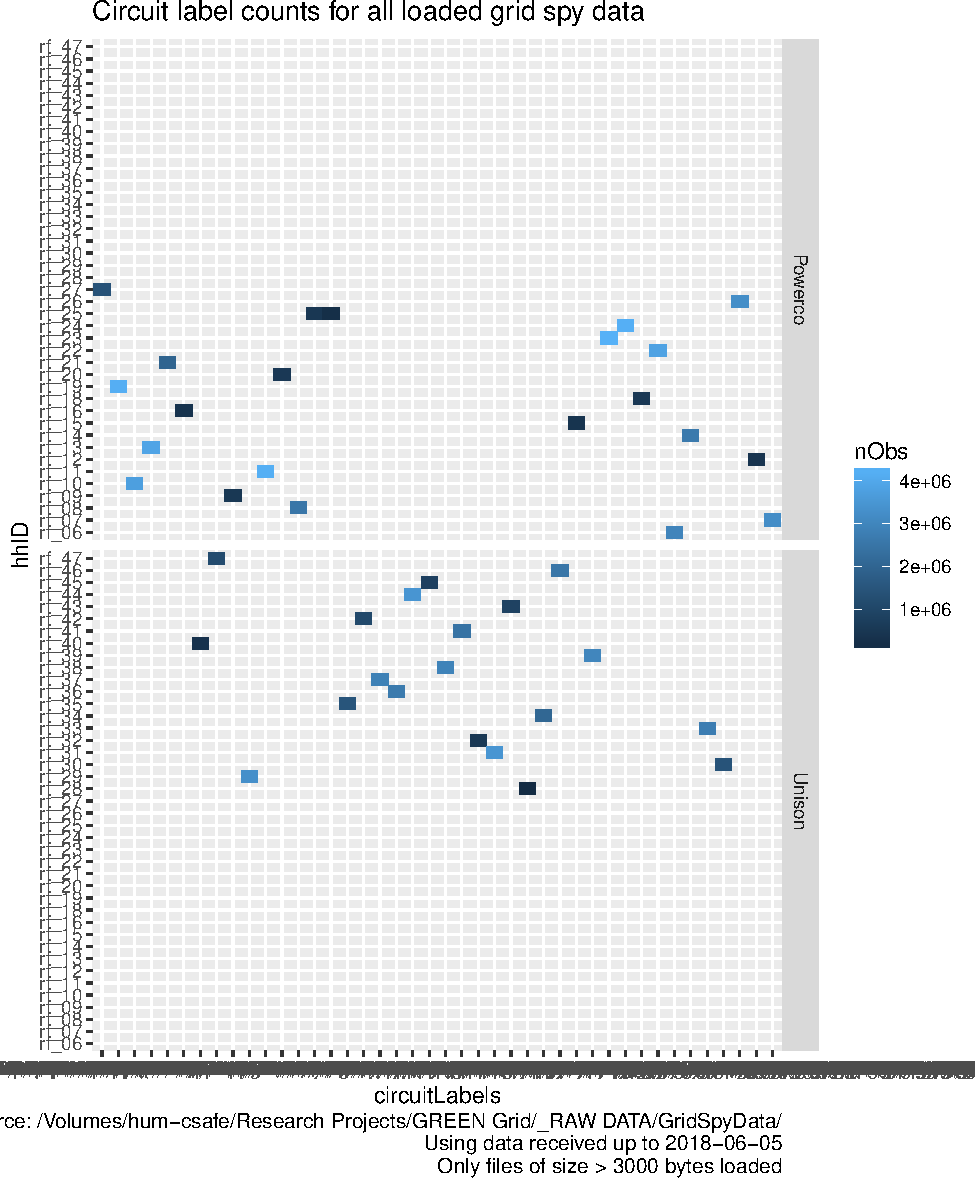
\includegraphics{processGridSpy1minData_files/figure-latex/plotCircuitLabelIssuesAsTile-1.pdf}

\begin{verbatim}
## Saving 6.5 x 8 in image
\end{verbatim}

The following table provides more detail to aid error checking. Check
for:

\begin{itemize}
\tightlist
\item
  2+ adjacent rows which have exactly the same circuit labels but
  different hh\_ids. This implies some data from one household has been
  saved in the wrong folder;
\item
  2+ adjacent rows which have different circuit labels but identical
  hh\_ids. This could imply the same thing but is more likely to be
  errors/changes to the circuit labelling.
\end{itemize}

If the above plot and this table flag a lot of errors then some
re-naming of the circuit labels (column names) may be necessary.

\begin{quote}
NB: As before, the table is only legible in the html version of this
report because latex does a very bad job of wrapping table cell text. A
version is saved in /Volumes/hum-csafe/Research Projects/GREEN
Grid/Clean\_data/safe/gridSpy/1min/circuitLabelMetaDataCheckTable.csv
for viewing in e.g.~xl.
\end{quote}

\begin{longtable}[]{@{}lllrllllr@{}}
\caption{Circuit labels by household with addiitonal
meta-data}\tabularnewline
\toprule
circuitLabels & hhID & sample & nFiles & minObsDate & maxObsDate &
minFileDate & maxFileDate & nObs\tabularnewline
\midrule
\endfirsthead
\toprule
circuitLabels & hhID & sample & nFiles & minObsDate & maxObsDate &
minFileDate & maxFileDate & nObs\tabularnewline
\midrule
\endhead
Bed 2, 2nd Fridge\$2828, Heat Pump\$2826, Hot Water - Controlled\$2825,
Incomer - Uncontrolled\$2824, Kitchen, Laundry \& Beds 1\&3\$2829, Oven
\& Oven Wall Appliances\$2827 & rf\_27 & Powerco & 3 & 2014-07-27 &
2016-05-13 & 2016-05-25 & 2016-09-21 & 1419097\tabularnewline
Bedroom \& Lounge Heat Pumps\$2741, Incomer 1 - All\$2738, Incomer 2 -
All\$2737, Kitchen Appliances\$2735, Laundry\$2734, Oven\$2736, PV
1\$2739, PV 2\$2733, Theatre Heat Pump\$2740 & rf\_19 & Powerco & 508 &
2014-07-14 & 2018-05-30 & 2016-05-25 & 2018-05-30 &
4173266\tabularnewline
Bedrooms \& Lounge\$2602, Heat Pump\$2598, Incomer - All\$2599, Kitchen
Appliances\$2601, Laundry \& Garage\$2597, Oven\$2600 & rf\_10 & Powerco
& 358 & 2014-07-08 & 2018-03-29 & 2016-05-25 & 2018-03-30 &
3734792\tabularnewline
Downstairs (inc 1 Heat Pump)\$2212, Hot Water - Controlled\$2208,
Incomer - Uncontrolled\$2209, Kitchen \& Laundry\$2213, Oven \&
Hob\$2210, Upstairs Heat Pumps\$2211 & rf\_13 & Powerco & 440 &
2014-06-05 & 2018-05-30 & 2016-05-25 & 2018-05-30 &
3896353\tabularnewline
Fridge\$2752, Heat Pump \& Washing Machine\$2750, Incomer - All\$2748,
Kitchen Appliances \& Garage\$2753, Lower Bedrooms \& Bathrooms\$2751,
Oven\$2749 & rf\_21 & Powerco & 4 & 2014-07-14 & 2016-07-01 & 2016-05-25
& 2016-10-12 & 1972512\tabularnewline
Hallway \& Washing Machine\$2683, Hot Water - Controlled\$2679, Incomer
1 - Uncont inc Oven\$2681, Incomer 2 - Uncont inc Stove\$2680, Kitchen
Appliances \& Bedrooms\$2684, Microwave \& Breadmaker\$2682 & rf\_16 &
Powerco & 1 & 2014-07-09 & 2015-03-25 & 2016-09-20 & 2016-09-20 &
373523\tabularnewline
Heat Pump \& 2 x Bathroom Heat\$4171, Incomer - All\$4170, Kitchen Power
\& Heat, Lounge\$4174, Laundry, Garage \& 2 Bedrooms\$4173,
Lighting\$4172, Wall Oven\$4169 & rf\_47 & Unison & 3 & 2015-03-24 &
2016-05-08 & 2016-05-25 & 2016-09-20 & 1180942\tabularnewline
Heat Pump \& Bedroom 2\$2731, Incomer 1 - Uncont - Inc Hob\$2729,
Incomer 2 - Uncont - Inc Oven\$2730, Kitchen Appliances\$2727,
Laundry\$2732, Lounge, Dining \& Bedrooms\$2728 & rf\_09 & Powerco & 2 &
2014-07-13 & 2015-07-16 & 2016-09-21 & 2016-09-21 &
529363\tabularnewline
Heat Pump \& Kitchen Appliances\$4186, Hot Water - Controlled\$4184,
Incomer - Uncontrolled\$4181, Laundry\$4185, Lighting\$4183, Oven\$4182
& rf\_29 & Unison & 505 & 2015-03-25 & 2018-05-30 & 2016-05-25 &
2018-05-30 & 3288151\tabularnewline
Heat Pump \& Lounge\$2590, Hob\$2589, Hot Water Cpbd Heater- Cont\$2586,
Incomer - Uncontrolled\$2585, Kitchen Appliances \& Laundry\$2588, Spa -
Uncontrolled\$2587 & rf\_11 & Powerco & 508 & 2014-07-07 & 2018-05-30 &
2016-05-25 & 2018-05-30 & 4189933\tabularnewline
Heat Pump \& Misc\$2107, Hob\$2109, Hot Water - Controlled\$2110,
Incomer 1 - Uncontrolled\$2112, Incomer 2 - Uncontrolled\$2111, Oven \&
Kitchen Appliances\$2108 & rf\_20 & Powerco & 2 & 2014-05-28 &
2015-06-11 & 2016-09-21 & 2016-09-21 & 545138\tabularnewline
Heat Pump (x2) \& Lounge Power\$4166, Hot Water - Controlled\$4167,
Incomer - Uncontrolled\$4168, Kitchen Appliances\$4163, Laundry\$4164,
Lighting\$4165 & rf\_40 & Unison & 2 & 2015-03-24 & 2015-11-22 &
2016-06-08 & 2016-09-20 & 349528\tabularnewline
Heat Pump\$2092, Hot Water - Controlled\$2094, Incomer -
Uncontrolled\$2093, Kitchen\$2089, Laundry \& 2nd Fridge Freezer\$2090,
Oven \& Hob\$2091 & rf\_08 & Powerco & 5 & 2014-05-28 & 2017-05-15 &
2016-05-25 & 2017-11-21 & 2536195\tabularnewline
Heat Pump\$2758, Hob \& Kitchen Appliances\$2759, Hot Water -
Controlled\$2761, Incomer 1 - Uncontrolled \$2763, Incomer 1 -
Uncontrolled\$2757, Incomer 2 - Uncontrolled \$2762, Oven\$2760 & rf\_25
& Powerco & 1 & 2015-05-24 & 2016-05-25 & 2016-06-08 & 2016-06-08 &
507847\tabularnewline
Heat Pump\$2758, Hob \& Kitchen Appliances\$2759, Hot Water -
Controlled\$2761, Incomer 1 - Uncontrolled \$2763, Incomer 2 -
Uncontrolled \$2762, Oven\$2760 & rf\_25 & Powerco & 2 & 2016-05-25 &
2016-10-22 & 2016-10-25 & 2017-11-21 & 213418\tabularnewline
Heat Pump\$4124, Hot Water - Uncontrolled\$4125, Incomer -
Uncontrolled\$4126, Kitchen Appliances\$4121, Laundry, Garage Fridge
Freezer\$4122, Lighting\$4123 & rf\_35 & Unison & 134 & 2015-03-22 &
2017-05-17 & 2016-05-25 & 2017-11-21 & 1494089\tabularnewline
Heat Pump\$4130, Hot Water - Uncontrolled\$4131, Incomer - All\$4132,
Kitchen Appliances\$4127, Laundry \& Freezer\$4128, Lighting (inc heat
lamps)\$4129 & rf\_42 & Unison & 45 & 2015-03-23 & 2017-02-18 &
2016-06-08 & 2017-11-21 & 1099072\tabularnewline
Heat Pump\$4134, Hot Water - Controlled\$4135, Incomer
-Uncontrolled\$4136, Kitchen Appliances\$4137, Laundry \& Fridge
Freezer\$4138, Lighting\$4133 & rf\_37 & Unison & 507 & 2015-03-23 &
2018-05-30 & 2016-06-08 & 2018-05-30 & 2849674\tabularnewline
Heat Pump\$4150, Hot Water - Uncontrolled\$4147, Incomer - All\$4148,
Kitchen Appliances\$4145, Lighting\$4149, Washing Machine\$4146 & rf\_36
& Unison & 458 & 2015-03-23 & 2018-05-30 & 2016-06-08 & 2018-05-30 &
2675600\tabularnewline
Heat Pump\$4154, Hot Water - Controlled\$4155, Incomer -
Uncontrolled\$4156, Kitchen Appliances\$4151, Laundry \$4152,
Lighting\$4153 & rf\_44 & Unison & 508 & 2015-03-24 & 2018-05-30 &
2016-05-25 & 2018-05-30 & 3464121\tabularnewline
Heat Pump\$4160, Hot Water - Controlled\$4158, Incomer -
Uncontrolled\$4157, Kitchen Appliances\$4161, Laundry \& Garage
Fridge\$4162, Lighting\$4159 & rf\_45 & Unison & 4 & 2015-03-24 &
2016-10-15 & 2016-06-08 & 2017-11-21 & 821472\tabularnewline
Heat Pump\$4175, Hot Water - Controlled\$4178, Incomer -
Uncontrolled\$4177, Kitchen, Dining \& Office\$4179, Laundry, Lounge,
Garage, Bed\$4180, Lighting\$4176 & rf\_38 & Unison & 402 & 2015-03-24 &
2017-08-22 & 2016-06-08 & 2017-11-21 & 2913338\tabularnewline
Heat Pump\$4190, Incomer - All\$4192, Kitchen Appliances\$4187,
Laundry\$4188, Lighting\$4189, Oven\$4191 & rf\_41 & Unison & 499 &
2015-03-25 & 2018-05-30 & 2016-06-08 & 2018-05-30 &
2441615\tabularnewline
Heat Pump\$4196, Hot Water - Controlled\$4198, Incomer - All\$4193,
Kitchen Appliances\$4195, Laundry\$4194, Lighting\$4197 & rf\_32 &
Unison & 2 & 2015-03-25 & 2016-04-05 & 2016-06-08 & 2016-09-20 &
542484\tabularnewline
Heat Pump\$4204, Hot Water - Controlled\$4200, Incomer - All\$4199,
Kitchen Appliances\$4201, Laundry\$4202, Lighting\$4203 & rf\_31 &
Unison & 508 & 2015-03-25 & 2018-05-30 & 2016-05-25 & 2018-05-30 &
3459721\tabularnewline
Heat Pump\$4211, Incomer - All\$4213, Kitchen Appliances\$4210, Laundry,
Garage \& Guest Bed\$4215, Lighting\$4212, Oven\$4214 & rf\_43 & Unison
& 4 & 2015-03-26 & 2015-10-18 & 2016-05-25 & 2016-09-28 &
890700\tabularnewline
Heat Pump\$4219, Incomer - All\$4221, Kitchen Appliances\$4216,
Laundry\$4217, Lighting\$4218, PV \& Garage\$4220 & rf\_28 & Unison & 2
& 2015-03-26 & 2015-05-26 & 2016-06-08 & 2016-09-19 &
87417\tabularnewline
Heat Pump\$4223, Hot Water - Uncontrolled\$4224, Incomer - All\$4225,
Kitchen Appliances\$4226, Laundry \& Garage Freezer\$4227,
Lighting\$4222 & rf\_34 & Unison & 7 & 2014-11-03 & 2016-08-24 &
2016-05-25 & 2016-10-13 & 2066074\tabularnewline
Heat Pumps (2x) \& Power\$4232, Heat Pumps (2x) \& Power\$4399, Hot
Water - Controlled\$4231, Hot Water - Controlled\$4400, Incomer -
Uncontrolled\$4230, Incomer - Uncontrolled\$4401, Incomer Voltage\$4405,
Kitchen \& Bedrooms\$4229, Kitchen \& Bedrooms\$4402, Laundry \&
Bedrooms\$4228, Laundry \& Bedrooms\$4403, Lighting\$4233,
Lighting\$4404 & rf\_46 & Unison & 411 & 2015-03-26 & 2018-02-19 &
2016-06-08 & 2018-02-21 & 2529107\tabularnewline
Hob\$3954, Hot Water\$3952, Incomer 1\$3956, Incomer 2\$3955, Laundry \&
Kitchen Appliances\$3951, Oven\$3953 & rf\_15 & Powerco & 2 & 2015-01-14
& 2016-04-18 & 2016-09-21 & 2016-09-21 & 395011\tabularnewline
Hot Water (2 elements)\$4247, Incomer - Uncontrolled\$4248, Kitchen
Appliances\$4244, Lighting \& 2 Towel Rail\$4245, Oven\$4246 & rf\_39 &
Unison & 384 & 2015-03-27 & 2018-05-30 & 2016-05-25 & 2018-05-30 &
3014770\tabularnewline
Hot Water - Controlled (HEMS)\$2081, Incomer - Uncontrolled\$2082,
Kitchen, Laundry \& Ventilation\$2084, Oven\$2085, PV \& Storage\$2083,
Spa (HEMS)\$2080 & rf\_23 & Powerco & 508 & 2014-05-25 & 2018-05-30 &
2016-05-25 & 2018-05-30 & 4253222\tabularnewline
Hot Water - Controlled\$2102, Incomer - Uncontrolled\$2101,
Kitchen\$2104, Laundry, Fridge \& Freezer\$2105, Oven \& Hob\$2103,
PV\$2106 & rf\_24 & Powerco & 508 & 2014-05-28 & 2018-05-30 & 2016-05-25
& 2018-05-30 & 4203991\tabularnewline
Hot Water - Controlled\$2129, Incomer 1 - Uncontrolled\$2128, Incomer 2
- Uncontrolled\$2130, Kitchen Appliances \& Ventilati\$2131, Laundry \&
Hob\$2133, Oven\$2132 & rf\_18 & Powerco & 2 & 2014-05-29 & 2015-06-11 &
2016-09-21 & 2016-09-21 & 543098\tabularnewline
Hot Water - Controlled\$2236, Incomer - Uncontrolled\$2237, Kitchen \&
Laundry\$2234, Lighting\$2232, Oven\$2235, Ventilation \& Lounge
Power\$2233 & rf\_22 & Powerco & 371 & 2014-06-05 & 2018-01-14 &
2016-05-25 & 2018-01-16 & 3837181\tabularnewline
Hot Water - Controlled\$2248, Incomer - Uncontrolled\$2249,
Kitchen\$2246, Laundry, Downstairs \& Lounge\$2245, Lighting\$2244, Oven
\& Hob\$2247 & rf\_06 & Powerco & 206 & 2014-06-08 & 2018-05-30 &
2016-05-25 & 2018-05-30 & 2964716\tabularnewline
Hot Water - Controlled\$2719, Incomer 1 - Uncont inc Stove\$2718,
Incomer 2 - Uncont inc Oven\$2717, Kitchen Appliances\$2715, Laundry \&
Microwave\$2720, Power Outlets\$2716 & rf\_14 & Powerco & 329 &
2014-07-13 & 2017-12-30 & 2016-06-08 & 2017-12-31 &
2654180\tabularnewline
Hot Water - Controlled\$4144, Incomer - Uncontrolled\$4143, Kitchen
Appliances \& Heat Pump\$4140, Laundry \& Teenagers Bedroom\$4139,
Lighting\$4142, Oven, Hob \& Microwave\$4141 & rf\_33 & Unison & 507 &
2015-03-23 & 2018-05-30 & 2016-06-08 & 2018-05-30 &
2749942\tabularnewline
Hot Water - Controlled\$4238, Incomer - All\$4239, Kitchen
Appliances\$4234, Laundry \& Kitchen\$4235, Lighting\$4236, Oven \&
Hobb\$4237 & rf\_30 & Unison & 5 & 2015-03-27 & 2016-09-29 & 2016-05-25
& 2016-10-13 & 1454037\tabularnewline
Incomer 1 - All\$2703, Incomer 2 - All\$2704, Kitchen Appliances\$2706,
Laundry, Sauna \& 2nd Fridge\$2707, Oven\$2705, Spa\$2708 & rf\_26 &
Powerco & 414 & 2014-07-10 & 2018-05-30 & 2016-05-25 & 2018-05-30 &
3239136\tabularnewline
Incomer 1 - Hot Water - Cont\$2626, Incomer 2 - Uncontrolled\$2625,
Incomer 3 - Uncontrolled\$2627, Kitchen Appliances \& Lounge\$2630,
Laundry, Fridge \& Microwave\$2628, Oven\$2629 & rf\_12 & Powerco & 2 &
2014-07-08 & 2015-06-02 & 2016-09-21 & 2016-09-21 &
410063\tabularnewline
Incomer 1 - Uncontrolled\$2726, Incomer 2 - Uncontrolled\$2725, Kitchen
Appliances \& Laundry\$2722, Microwave\$2721, Oven\$2724, Workshop\$2723
& rf\_07 & Powerco & 206 & 2014-07-13 & 2018-05-30 & 2016-05-25 &
2018-05-30 & 3216449\tabularnewline
\bottomrule
\end{longtable}

Things to note:

\begin{itemize}
\tightlist
\item
  rf\_25 has an aditional unexpected ``Incomer 1 - Uncontrolled\$2757''
  circuit in some files but it's value is always NA so we have not
  `corrected' this.
\end{itemize}

\subsection{Observations}\label{observations}

The following plots show the number of observations per day per
household. In theory we should not see:

\begin{itemize}
\tightlist
\item
  dates before 2014 or in to the future. These may indicate:

  \begin{itemize}
  \tightlist
  \item
    date conversion errors;
  \end{itemize}
\item
  more than 1440 observations per day. These may indicate:

  \begin{itemize}
  \tightlist
  \item
    duplicate time stamps - i.e.~they have the same time stamps but
    different power (W) values or different circuit labels;
  \item
    observations from files that are in the `wrong' rf\_XX folder and so
    are included in the `wrong' household as `duplicate' time stamps.
  \end{itemize}
\end{itemize}

If present both of the latter may have been implied by the table above
and would have evaded the de-duplication filter which simply checks each
complete row against all others within it's consolidated household
dataset (a \emph{within household absolute duplicate} check).

\begin{verbatim}
## Warning: Removed 3 rows containing missing values (geom_tile).
\end{verbatim}

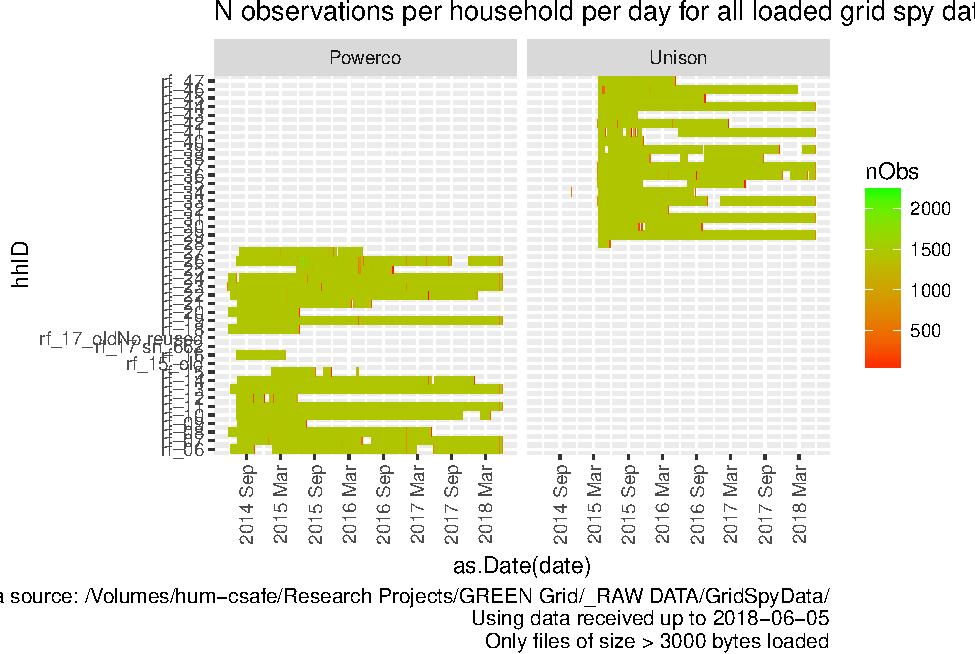
\includegraphics{processGridSpy1minData_files/figure-latex/loadedFilesObsPlots-1.pdf}

\begin{verbatim}
## Saving 6.5 x 4.5 in image
\end{verbatim}

\begin{verbatim}
## Warning: Removed 3 rows containing missing values (geom_tile).
\end{verbatim}

\begin{verbatim}
## Warning: Removed 3 rows containing missing values (geom_point).
\end{verbatim}

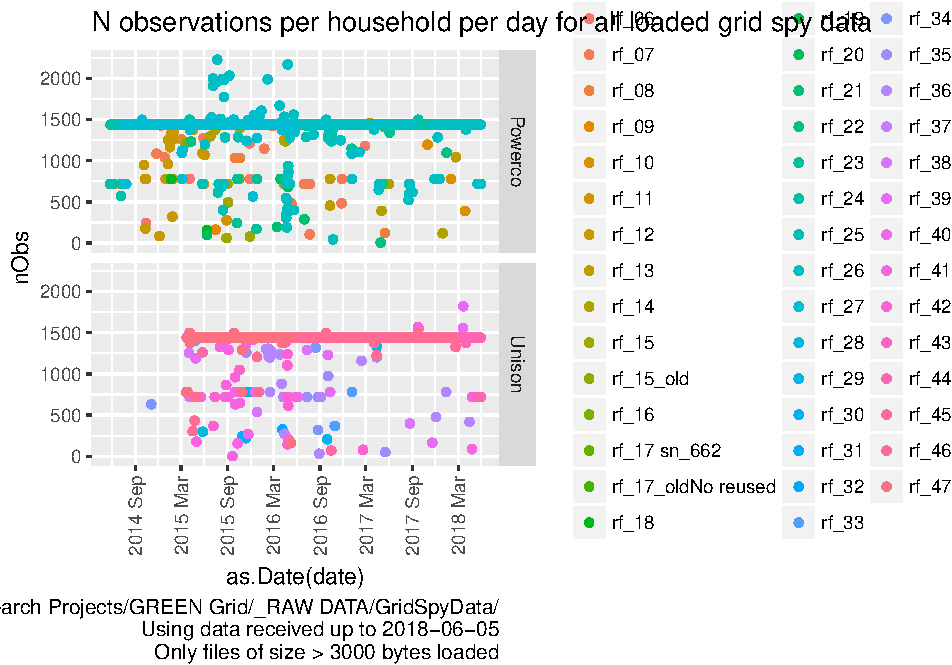
\includegraphics{processGridSpy1minData_files/figure-latex/plot n obs per hh id as dots-1.pdf}

\begin{verbatim}
## Saving 6.5 x 4.5 in image
\end{verbatim}

\begin{verbatim}
## Warning: Removed 3 rows containing missing values (geom_point).
\end{verbatim}

The following table shows the min/max observations per day and min/max
dates for each household. As above, we should not see:

\begin{itemize}
\tightlist
\item
  dates before 2014 or in to the future (indicates date conversion
  errors)
\item
  more than 1440 observations per day (indicates potentially duplicate
  observations)
\item
  non-integer counts of circuits as it suggests some column errors
\end{itemize}

We should also not see NA in any row (indicates date conversion errors).

If we do see any of these then we still have data cleaning work to do!

\begin{longtable}[]{@{}llrrrll@{}}
\caption{Summary observation stats by hhID (sorted by date last heard
from)}\tabularnewline
\toprule
hhID & sample & minObs & maxObs & meanNDataColumns & minDate &
maxDate\tabularnewline
\midrule
\endfirsthead
\toprule
hhID & sample & minObs & maxObs & meanNDataColumns & minDate &
maxDate\tabularnewline
\midrule
\endhead
rf\_16 & Powerco & 720 & 1500 & 6 & 2014-07-09 &
2015-03-25\tabularnewline
rf\_28 & Unison & 297 & 1440 & 6 & 2015-03-26 &
2015-05-26\tabularnewline
rf\_12 & Powerco & 85 & 1500 & 6 & 2014-07-08 &
2015-06-02\tabularnewline
rf\_18 & Powerco & 157 & 1500 & 6 & 2014-05-29 &
2015-06-11\tabularnewline
rf\_20 & Powerco & 98 & 1500 & 6 & 2014-05-28 &
2015-06-11\tabularnewline
rf\_09 & Powerco & 163 & 1500 & 6 & 2014-07-13 &
2015-07-16\tabularnewline
rf\_43 & Unison & 780 & 1495 & 6 & 2015-03-26 &
2015-10-18\tabularnewline
rf\_40 & Unison & 268 & 1500 & 6 & 2015-03-24 &
2015-11-22\tabularnewline
rf\_32 & Unison & 325 & 1500 & 6 & 2015-03-25 &
2016-04-05\tabularnewline
rf\_15 & Powerco & 62 & 1440 & 6 & 2015-01-14 &
2016-04-18\tabularnewline
rf\_47 & Unison & 159 & 1500 & 6 & 2015-03-24 &
2016-05-08\tabularnewline
rf\_27 & Powerco & 567 & 1560 & 6 & 2014-07-27 &
2016-05-13\tabularnewline
rf\_21 & Powerco & 195 & 1500 & 6 & 2014-07-14 &
2016-07-01\tabularnewline
rf\_34 & Unison & 317 & 1500 & 6 & 2014-11-03 &
2016-08-24\tabularnewline
rf\_30 & Unison & 205 & 1500 & 6 & 2015-03-27 &
2016-09-29\tabularnewline
rf\_45 & Unison & 69 & 1499 & 6 & 2015-03-24 & 2016-10-15\tabularnewline
rf\_25 & Powerco & 45 & 1500 & 6 & 2015-05-24 &
2016-10-22\tabularnewline
rf\_42 & Unison & 79 & 1500 & 6 & 2015-03-23 & 2017-02-18\tabularnewline
rf\_08 & Powerco & 123 & 1500 & 6 & 2014-05-28 &
2017-05-15\tabularnewline
rf\_35 & Unison & 50 & 1500 & 6 & 2015-03-22 & 2017-05-17\tabularnewline
rf\_38 & Unison & 398 & 1500 & 6 & 2015-03-24 &
2017-08-22\tabularnewline
rf\_14 & Powerco & 120 & 1500 & 6 & 2014-07-13 &
2017-12-30\tabularnewline
rf\_22 & Powerco & 6 & 1500 & 6 & 2014-06-05 & 2018-01-14\tabularnewline
rf\_46 & Unison & 305 & 1500 & 13 & 2015-03-26 &
2018-02-19\tabularnewline
rf\_10 & Powerco & 389 & 1500 & 6 & 2014-07-08 &
2018-03-29\tabularnewline
rf\_06 & Powerco & 243 & 1500 & 6 & 2014-06-08 &
2018-05-30\tabularnewline
rf\_07 & Powerco & 105 & 1500 & 6 & 2014-07-13 &
2018-05-30\tabularnewline
rf\_11 & Powerco & 278 & 1500 & 6 & 2014-07-07 &
2018-05-30\tabularnewline
rf\_13 & Powerco & 456 & 1500 & 6 & 2014-06-05 &
2018-05-30\tabularnewline
rf\_19 & Powerco & 387 & 1500 & 9 & 2014-07-14 &
2018-05-30\tabularnewline
rf\_23 & Powerco & 171 & 1500 & 6 & 2014-05-25 &
2018-05-30\tabularnewline
rf\_24 & Powerco & 571 & 1500 & 6 & 2014-05-28 &
2018-05-30\tabularnewline
rf\_26 & Powerco & 362 & 2231 & 6 & 2014-07-10 &
2018-05-30\tabularnewline
rf\_29 & Unison & 720 & 1500 & 6 & 2015-03-25 &
2018-05-30\tabularnewline
rf\_31 & Unison & 720 & 1500 & 6 & 2015-03-25 &
2018-05-30\tabularnewline
rf\_33 & Unison & 369 & 1500 & 6 & 2015-03-23 &
2018-05-30\tabularnewline
rf\_36 & Unison & 29 & 1500 & 6 & 2015-03-23 & 2018-05-30\tabularnewline
rf\_37 & Unison & 720 & 1500 & 6 & 2015-03-23 &
2018-05-30\tabularnewline
rf\_39 & Unison & 163 & 1823 & 5 & 2015-03-27 &
2018-05-30\tabularnewline
rf\_41 & Unison & 1 & 1573 & 6 & 2015-03-25 & 2018-05-30\tabularnewline
rf\_44 & Unison & 720 & 1500 & 6 & 2015-03-24 &
2018-05-30\tabularnewline
rf\_15\_old & Powerco & NA & NA & NA & NA & NA\tabularnewline
rf\_17 sn\_662 & Powerco & NA & NA & NA & NA & NA\tabularnewline
rf\_17\_oldNo reused & Powerco & NA & NA & NA & NA & NA\tabularnewline
\bottomrule
\end{longtable}

Finally we show the total number of households which we think are still
sending data.

\begin{verbatim}
## Warning: Removed 1 rows containing missing values (position_stack).
\end{verbatim}

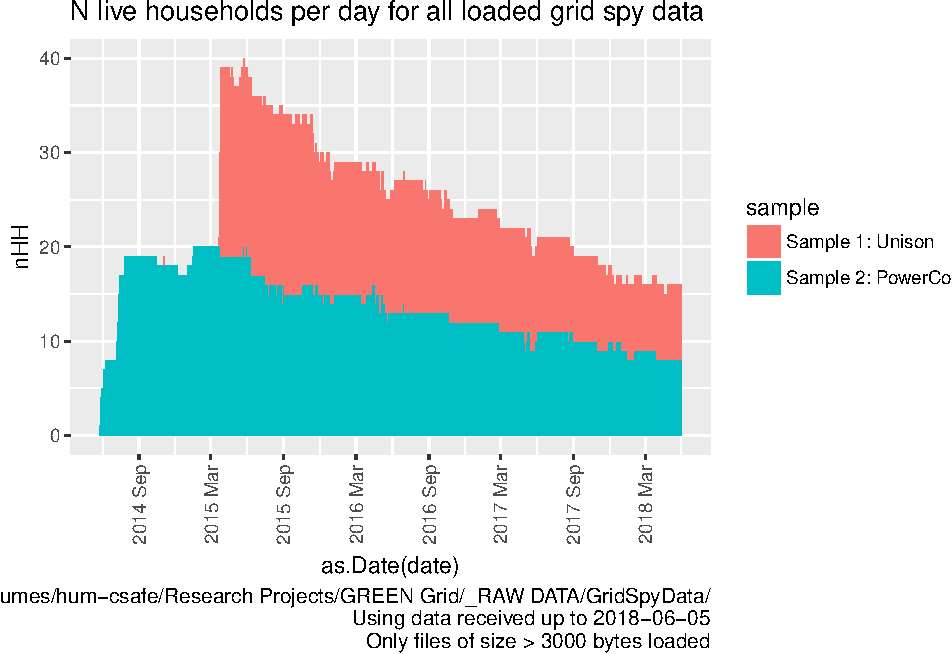
\includegraphics{processGridSpy1minData_files/figure-latex/liveDataHouseholds-1.pdf}

\begin{verbatim}
## Saving 6.5 x 4.5 in image
\end{verbatim}

\begin{verbatim}
## Warning: Removed 1 rows containing missing values (position_stack).
\end{verbatim}

\section{Summary}\label{summary}

The cleaned data has been saved as gzipped .csv files to
/Volumes/hum-csafe/Research Projects/GREEN
Grid/Clean\_data/safe/gridSpy/1min/ in `long' form so that each file
only has 4 columns:

\begin{itemize}
\tightlist
\item
  hhID: household id
\item
  r\_dateTime: time of observation
\item
  circuit: the circuit label
\item
  powerW: power observation (Watts)
\end{itemize}

Each file has data for one household and there should be one file per
household.

As an example, here are the first few rows of one of the files:

\begin{longtable}[]{@{}lllr@{}}
\caption{Example data rows}\tabularnewline
\toprule
hhID & r\_dateTime & circuit & powerW\tabularnewline
\midrule
\endfirsthead
\toprule
hhID & r\_dateTime & circuit & powerW\tabularnewline
\midrule
\endhead
rf\_01 & 2014-01-06 03:03:00 & Kitchen power\$1632 &
45.58\tabularnewline
rf\_01 & 2014-01-06 03:04:00 & Kitchen power\$1632 &
45.58\tabularnewline
rf\_01 & 2014-03-07 02:56:00 & Kitchen power\$1632 &
45.58\tabularnewline
rf\_01 & 2014-03-07 02:57:00 & Kitchen power\$1632 &
54.13\tabularnewline
rf\_01 & 2014-03-07 02:58:00 & Kitchen power\$1632 &
136.26\tabularnewline
rf\_01 & 2014-03-07 02:59:00 & Kitchen power\$1632 &
141.96\tabularnewline
\bottomrule
\end{longtable}

This format makes it much easier to do future data extraction in R as we
can select by date and circuit label as we load. It also means we can
load a lot of data in memory without breaking R's memory limits as R
likes `long' rather than wide data.

\section{Runtime}\label{runtime}

Analysis completed in 35.3 seconds ( 0.59 minutes) using
\href{https://cran.r-project.org/package=knitr}{knitr} in
\href{http://www.rstudio.com}{RStudio} with R version 3.5.0 (2018-04-23)
running on x86\_64-apple-darwin15.6.0.

The time taken will have depended on:

\begin{quote}
Full run using all data from /Volumes/hum-csafe/Research Projects/GREEN
Grid/\_RAW DATA/GridSpyData/
\end{quote}

\begin{quote}
refreshData = 0 so re-using previous output. Should be relatively quick.
\end{quote}

\section{R environment}\label{r-environment}

R packages used:

\begin{itemize}
\tightlist
\item
  base R - for the basics (R Core Team 2016)
\item
  data.table - for fast (big) data handling (Dowle et al. 2015)
\item
  lubridate - date manipulation (Grolemund and Wickham 2011)
\item
  ggplot2 - for slick graphics (Wickham 2009)
\item
  readr - for csv reading/writing (Wickham, Hester, and Francois 2016)
\item
  dplyr - for select and contains (Wickham and Francois 2016)
\item
  progress - for progress bars (Csárdi and FitzJohn 2016)
\item
  knitr - to create this document \& neat tables (Xie 2016)
\item
  kableExtra - for extra neat tables (Zhu 2018)
\item
  nzGREENGrid - for local NZ GREEN Grid project utilities
\end{itemize}

Session info:

\begin{verbatim}
## R version 3.5.0 (2018-04-23)
## Platform: x86_64-apple-darwin15.6.0 (64-bit)
## Running under: macOS High Sierra 10.13.4
## 
## Matrix products: default
## BLAS: /Library/Frameworks/R.framework/Versions/3.5/Resources/lib/libRblas.0.dylib
## LAPACK: /Library/Frameworks/R.framework/Versions/3.5/Resources/lib/libRlapack.dylib
## 
## locale:
## [1] en_GB.UTF-8/en_GB.UTF-8/en_GB.UTF-8/C/en_GB.UTF-8/en_GB.UTF-8
## 
## attached base packages:
## [1] stats     graphics  grDevices utils     datasets  methods   base     
## 
## other attached packages:
## [1] knitr_1.20        readr_1.1.1       ggplot2_2.2.1     data.table_1.11.2
## [5] nzGREENGrid_0.1.0
## 
## loaded via a namespace (and not attached):
##  [1] Rcpp_0.12.17      cellranger_1.1.0  highr_0.6        
##  [4] pillar_1.2.2      compiler_3.5.0    plyr_1.8.4       
##  [7] bindr_0.1.1       prettyunits_1.0.2 tools_3.5.0      
## [10] progress_1.1.2    digest_0.6.15     lubridate_1.7.4  
## [13] evaluate_0.10.1   tibble_1.4.2      gtable_0.2.0     
## [16] pkgconfig_2.0.1   rlang_0.2.0       yaml_2.1.19      
## [19] bindrcpp_0.2.2    dplyr_0.7.5       stringr_1.3.1    
## [22] hms_0.4.2         rprojroot_1.3-2   grid_3.5.0       
## [25] tidyselect_0.2.4  glue_1.2.0        R6_2.2.2         
## [28] readxl_1.1.0      rmarkdown_1.9     purrr_0.2.4      
## [31] reshape2_1.4.3    magrittr_1.5      backports_1.1.2  
## [34] scales_0.5.0      htmltools_0.3.6   assertthat_0.2.0 
## [37] colorspace_1.3-2  labeling_0.3      stringi_1.2.2    
## [40] lazyeval_0.2.1    munsell_0.4.3
\end{verbatim}

\section*{References}\label{references}
\addcontentsline{toc}{section}{References}

\hypertarget{refs}{}
\hypertarget{ref-progress}{}
Csárdi, Gábor, and Rich FitzJohn. 2016. \emph{Progress: Terminal
Progress Bars}. \url{https://CRAN.R-project.org/package=progress}.

\hypertarget{ref-data.table}{}
Dowle, M, A Srinivasan, T Short, S Lianoglou with contributions from R
Saporta, and E Antonyan. 2015. \emph{Data.table: Extension of
Data.frame}. \url{https://CRAN.R-project.org/package=data.table}.

\hypertarget{ref-lubridate}{}
Grolemund, Garrett, and Hadley Wickham. 2011. ``Dates and Times Made
Easy with lubridate.'' \emph{Journal of Statistical Software} 40 (3):
1--25. \url{http://www.jstatsoft.org/v40/i03/}.

\hypertarget{ref-baseR}{}
R Core Team. 2016. \emph{R: A Language and Environment for Statistical
Computing}. Vienna, Austria: R Foundation for Statistical Computing.
\url{https://www.R-project.org/}.

\hypertarget{ref-ggplot2}{}
Wickham, Hadley. 2009. \emph{Ggplot2: Elegant Graphics for Data
Analysis}. Springer-Verlag New York. \url{http://ggplot2.org}.

\hypertarget{ref-dplyr}{}
Wickham, Hadley, and Romain Francois. 2016. \emph{Dplyr: A Grammar of
Data Manipulation}. \url{https://CRAN.R-project.org/package=dplyr}.

\hypertarget{ref-readr}{}
Wickham, Hadley, Jim Hester, and Romain Francois. 2016. \emph{Readr:
Read Tabular Data}. \url{https://CRAN.R-project.org/package=readr}.

\hypertarget{ref-knitr}{}
Xie, Yihui. 2016. \emph{Knitr: A General-Purpose Package for Dynamic
Report Generation in R}. \url{https://CRAN.R-project.org/package=knitr}.

\hypertarget{ref-kableExtra}{}
Zhu, Hao. 2018. \emph{KableExtra: Construct Complex Table with 'Kable'
and Pipe Syntax}. \url{https://CRAN.R-project.org/package=kableExtra}.


\end{document}
